\section{CIR- model}
\subsection{Calibration Parameters}
	\newcommand{\phiOneXA}{0.710501}
\newcommand{\phiTwoXA}{0.644564}
\newcommand{\phiThreeXA}{1.60862}
\newcommand{\xZeroA}{0.268914}
\newcommand{\phiOneYA}{0.468673}
\newcommand{\phiTwoYA}{0.533206}
\newcommand{\phiThreeYA}{1.50249}
\newcommand{\yZeroA}{0.280095}
\newcommand{\errFminA}{3.247465e-04}
\newcommand{\MREA}{0.144\,\%}
\newcommand{\MSREA}{0.001\,\%}
\newcommand{\cirParamTableA}{
\begin{tabular}{@{}*{8}{c}@{}}
$\phi_1^x$ & $\phi_2^x$ & $\phi_3^x$ & $x_0$ & $\phi_1^y$ & $\phi_2^y$ & $\phi_3^y$ & $y_0$\\
$\phiOneXA$ & $\phiTwoXA$ & $\phiThreeXA$ & $\xZeroA$ & $\phiOneYA$ & $\phiTwoYA$ & $\phiThreeYA$ & $\yZeroA$ \\
\end{tabular}
}
\newcommand{\cirErrorTableA}{
\begin{tabular}{@{}*{3}{c}@{}}
$f(\Pi)$ & \textbf{MRE} & \textbf{MSRE} \\
 $\errFminA$ & $\MREA$ & $\MSREA$
\end{tabular}
}
%\begin{tabular}{@{}*{9}{c}@{}}
%$\phi_1^x$ & $\phi_2^x$ & $\phi_3^x$ & $x_0$ & $\phi_1^y$ & $\phi_2^y$ & $\phi_3^y$ & $y_0$ & Error\\
%$0.710501$ & $0.644564$ & $1.60862$ & $0.468673$ &$0.533206$ & $1.50249$ & $0.268914$ & $0.280095$ & $%\end{tabular}

	\cirParamTableA\hfill\\
	\cirErrorTableA\hfill\\
\subsection{Model Parameters}
	\newcommand{\kXA}{0.578626}
\newcommand{\sigmaXA}{0.291551}
\newcommand{\thetaXA}{0.118155}
\newcommand{\kYA}{0.59774}
\newcommand{\sigmaYA}{0.262334}
\newcommand{\thetaYA}{0.0864925}
\newcommand{\modelParamTableA}{
\begin{tabular}{@{}*{6}{c}@{}}
$k_x$ & $\sigma_x$ & $\theta_x$ & $k_y$ & $\sigma_y$ & $\theta_y$ \\
$\kXA$ & $\sigmaXA$ & $\thetaXA$ & $\kYA$ & $\sigmaYA$ & $\thetaYA$ \\
\end{tabular}
}
%\begin{tabular}{@{}*{6}{c}@{}}
%$k_x$ & $\sigma_x$ & $\theta_x$ & $k_y$ & $\sigma_y$ & $\theta_y$ \\
%$0.578626$ & $0.291551$ & $0.118155$ & $0.59774$ & $0.262334$ & $0.0864925$ \\
%\end{tabular}

	\modelParamTableA
\subsection{Euler Parameter}
	\newcommand{\simulationsA}{10000}
\newcommand{\timeMeshA}{\frac{1}{256}}
\newcommand{\eulerParamA}{
We used $M=\simulationsA$ simulations and a mesh of $\Delta=\timeMeshA$
}

	\eulerParamA
\subsection{Computational Times}
	\SaveVerb{ga}=ga=
\SaveVerb{fmin}=fmin=
\newcommand{\ctimeA}{
\renewcommand{\arraystretch}{1}
\begin{tabular}{@{}*{3}{c}@{}}
Time \UseVerb{ga} (in s)& Time \UseVerb{fmin} (in s) & Time for simulations (in s)\\
$-1$ & $0.149811$ & $9.8687$ 
\end{tabular}
}

	\ctimeA
\hfill\\
	\newcommand{\ctimeTestsA}{
\renewcommand{\arraystretch}{1}
\begin{tabular}{c*{3}{c}}
Inital Parameter & Times (in s) & MRE (in \%) \\
\hline
\UseVerb{ga} &$42.136$ &$0.142014\,\%$\\
0.50001     0.50001         1.5     0.50001     0.50001         1.5     0.50001     0.50001 &$0.287$ &$0.143798\,\%$\\
1  1  2  1  1  2  1  1 &$0.229$ &$0.146769\,\%$\\
1e-05       1e-05           1       1e-05       1e-05           1       1e-05       1e-05 &$0.276$ &$0.145207\,\%$\\
0.048808     0.72079      1.4275     0.64469     0.32152      1.4794      0.2556     0.25427 &$0.334$ &$0.146509\,\%$\\
0.66073     0.78158      1.5547      0.3779     0.24209       1.249     0.74017     0.63334 &$103.949$ &$0.14374\,\%$
\end{tabular}
}
\newcommand{\ctimeTestsABody}{
\UseVerb{ga} &$42.136$ &$0.142014\,\%$\\
0.50001     0.50001         1.5     0.50001     0.50001         1.5     0.50001     0.50001 &$0.287$ &$0.143798\,\%$\\
1  1  2  1  1  2  1  1 &$0.229$ &$0.146769\,\%$\\
1e-05       1e-05           1       1e-05       1e-05           1       1e-05       1e-05 &$0.276$ &$0.145207\,\%$\\
0.048808     0.72079      1.4275     0.64469     0.32152      1.4794      0.2556     0.25427 &$0.334$ &$0.146509\,\%$\\
0.66073     0.78158      1.5547      0.3779     0.24209       1.249     0.74017     0.63334 &$103.949$ &$0.14374\,\%$
}
\newcommand{\ctimeTestsAHeader}{
Inital Parameter & Times (in s) & MRE (in \%) \\
}
\newcommand{\ctimeTestsAData}{
$42.136$ &$0.142014\,\%$\\
$0.287$ &$0.143798\,\%$\\
$0.229$ &$0.146769\,\%$\\
$0.276$ &$0.145207\,\%$\\
$0.334$ &$0.146509\,\%$\\
$103.949$ &$0.14374\,\%$
}
\newcommand{\ctimeTestsADescription}{
\UseVerb{ga}\\
0.50001     0.50001         1.5     0.50001     0.50001         1.5     0.50001     0.50001\\
1  1  2  1  1  2  1  1\\
1e-05       1e-05           1       1e-05       1e-05           1       1e-05       1e-05\\
0.048808     0.72079      1.4275     0.64469     0.32152      1.4794      0.2556     0.25427\\
0.66073     0.78158      1.5547      0.3779     0.24209       1.249     0.74017     0.63334
}

	\ctimeTestsA
\subsection{Mean errors of Discount Factor}
	\newcommand{\dfMeanErrA}{
\renewcommand{\arraystretch}{1}
\begin{tabular}{@{}*{2}{c}@{}}
Maturity (in years) & Mean Error of Discount Factor\\
\hline
$0.0833333$ & $0.000409963$ \\
$0.25$ & $0.00112268$ \\
$0.5$ & $0.00161849$ \\
$0.75$ & $0.00137477$ \\
$1$ & $0.000814101$ \\
$1.25$ & $0.000328491$ \\
$1.5$ & $1.4362e-05$ \\
$1.75$ & $5.62967e-05$ \\
$2$ & $0.000402274$ \\
$2.25$ & $0.000824884$ \\
$2.5$ & $0.0011063$ \\
$2.75$ & $0.00133005$ \\
$3$ & $0.00143482$ \\
$3.25$ & $0.0018223$ \\
$3.5$ & $0.00242705$ \\
$3.75$ & $0.00303645$ \\
$4$ & $0.00354305$ \\
$4.25$ & $0.00409665$ \\
$4.5$ & $0.00461513$ \\
$4.75$ & $0.00491301$ \\
$5$ & $0.00502117$ \\
$5.25$ & $0.00485501$ \\
$5.5$ & $0.0048752$ \\
$5.75$ & $0.00549422$ \\
$6$ & $0.00642713$ \\
$6.25$ & $0.00743045$ \\
$6.5$ & $0.00841358$ \\
$6.75$ & $0.00945159$ \\
$7$ & $0.010154$ \\
$7.25$ & $0.0105884$ \\
$7.5$ & $0.0111652$ \\
$7.75$ & $0.0116295$ \\
$8$ & $0.0120698$ \\
$8.25$ & $0.0125788$ \\
$8.5$ & $0.0132799$ \\
$8.75$ & $0.0138392$ \\
$9$ & $0.0146873$ \\
$9.25$ & $0.0156794$ \\
$9.5$ & $0.0166502$ \\
$9.75$ & $0.0174248$ \\
$10$ & $0.0180652$ \\
$15$ & $0.0251373$ \\
$20$ & $0.0331911$ \\
$25$ & $0.0160001$ \\
$30$ & $0.00094742$ 
\end{tabular}
}
\newcommand{\dfMeanErrABody}{
$0.0833333$ & $0.000409963$ \\
$0.25$ & $0.00112268$ \\
$0.5$ & $0.00161849$ \\
$0.75$ & $0.00137477$ \\
$1$ & $0.000814101$ \\
$1.25$ & $0.000328491$ \\
$1.5$ & $1.4362e-05$ \\
$1.75$ & $5.62967e-05$ \\
$2$ & $0.000402274$ \\
$2.25$ & $0.000824884$ \\
$2.5$ & $0.0011063$ \\
$2.75$ & $0.00133005$ \\
$3$ & $0.00143482$ \\
$3.25$ & $0.0018223$ \\
$3.5$ & $0.00242705$ \\
$3.75$ & $0.00303645$ \\
$4$ & $0.00354305$ \\
$4.25$ & $0.00409665$ \\
$4.5$ & $0.00461513$ \\
$4.75$ & $0.00491301$ \\
$5$ & $0.00502117$ \\
$5.25$ & $0.00485501$ \\
$5.5$ & $0.0048752$ \\
$5.75$ & $0.00549422$ \\
$6$ & $0.00642713$ \\
$6.25$ & $0.00743045$ \\
$6.5$ & $0.00841358$ \\
$6.75$ & $0.00945159$ \\
$7$ & $0.010154$ \\
$7.25$ & $0.0105884$ \\
$7.5$ & $0.0111652$ \\
$7.75$ & $0.0116295$ \\
$8$ & $0.0120698$ \\
$8.25$ & $0.0125788$ \\
$8.5$ & $0.0132799$ \\
$8.75$ & $0.0138392$ \\
$9$ & $0.0146873$ \\
$9.25$ & $0.0156794$ \\
$9.5$ & $0.0166502$ \\
$9.75$ & $0.0174248$ \\
$10$ & $0.0180652$ \\
$15$ & $0.0251373$ \\
$20$ & $0.0331911$ \\
$25$ & $0.0160001$ \\
$30$ & $0.00094742$ 
}
\newcommand{\dfMeanErrAHeader}{
Maturity (in years) & Mean Error of Discount Factor\\
}
\newcommand{\dfMeanErrAData}{
$0.000409963$ \\
$0.00112268$ \\
$0.00161849$ \\
$0.00137477$ \\
$0.000814101$ \\
$0.000328491$ \\
$1.4362e-05$ \\
$5.62967e-05$ \\
$0.000402274$ \\
$0.000824884$ \\
$0.0011063$ \\
$0.00133005$ \\
$0.00143482$ \\
$0.0018223$ \\
$0.00242705$ \\
$0.00303645$ \\
$0.00354305$ \\
$0.00409665$ \\
$0.00461513$ \\
$0.00491301$ \\
$0.00502117$ \\
$0.00485501$ \\
$0.0048752$ \\
$0.00549422$ \\
$0.00642713$ \\
$0.00743045$ \\
$0.00841358$ \\
$0.00945159$ \\
$0.010154$ \\
$0.0105884$ \\
$0.0111652$ \\
$0.0116295$ \\
$0.0120698$ \\
$0.0125788$ \\
$0.0132799$ \\
$0.0138392$ \\
$0.0146873$ \\
$0.0156794$ \\
$0.0166502$ \\
$0.0174248$ \\
$0.0180652$ \\
$0.0251373$ \\
$0.0331911$ \\
$0.0160001$ \\
$0.00094742$ 
}

\begin{table}
	\dfMeanErrA
\centering
\caption{Market data containing the zero rate curve and zero coupon curve at 30/12/2019.}
\label{tab:market_dataA}
\end{table}
\subsection{Errors of Swaption}
	\newcommand{\errorSwaptionA}{
\renewcommand{\arraystretch}{1}
\begin{tabular}{|c|*{5}{c}|}
\hline
\diagbox{Maturity}{Tenor} & 1 & 2 & 5 & 7 & 10 \\
 \hline
$1$ & $4.82602\,\% $ & $3.72741\,\% $ & $1.56009\,\% $ & $0.601718\,\% $ & $-0.554628\,\% $ \\
$2$ & $4.70047\,\% $ & $3.56775\,\% $ & $1.18057\,\% $ & $0.0467543\,\% $ & $-1.37405\,\% $ \\
$5$ & $3.60511\,\% $ & $2.4125\,\% $ & $-0.249531\,\% $ & $-1.64559\,\% $ & $-3.50471\,\% $ \\
$7$ & $3.23362\,\% $ & $1.97696\,\% $ & $-0.945175\,\% $ & $-2.48803\,\% $ & $-4.54551\,\% $ \\
$10$ & $2.85895\,\% $ & $1.49467\,\% $ & $-1.69265\,\% $ & $-3.37829\,\% $ & $-5.63478\,\% $ \\
$15$ & $2.63259\,\% $ & $1.17927\,\% $ & $-2.21714\,\% $ & $-4.05043\,\% $ & $-6.53224\,\% $ \\
$20$ & $2.48029\,\% $ & $1.01554\,\% $ & $-2.47166\,\% $ & $-4.39298\,\% $ & $-6.98019\,\% $ 
\\\hline
\end{tabular}
}

\begin{table}
	\errorSwaptionA
\centering
\caption{Swaption error for data at 30/12/2019.}
\label{tab:swaption_errorA}
\end{table}
\subsection{Plots of Zero Coupon Prices}
	\begin{landscape}
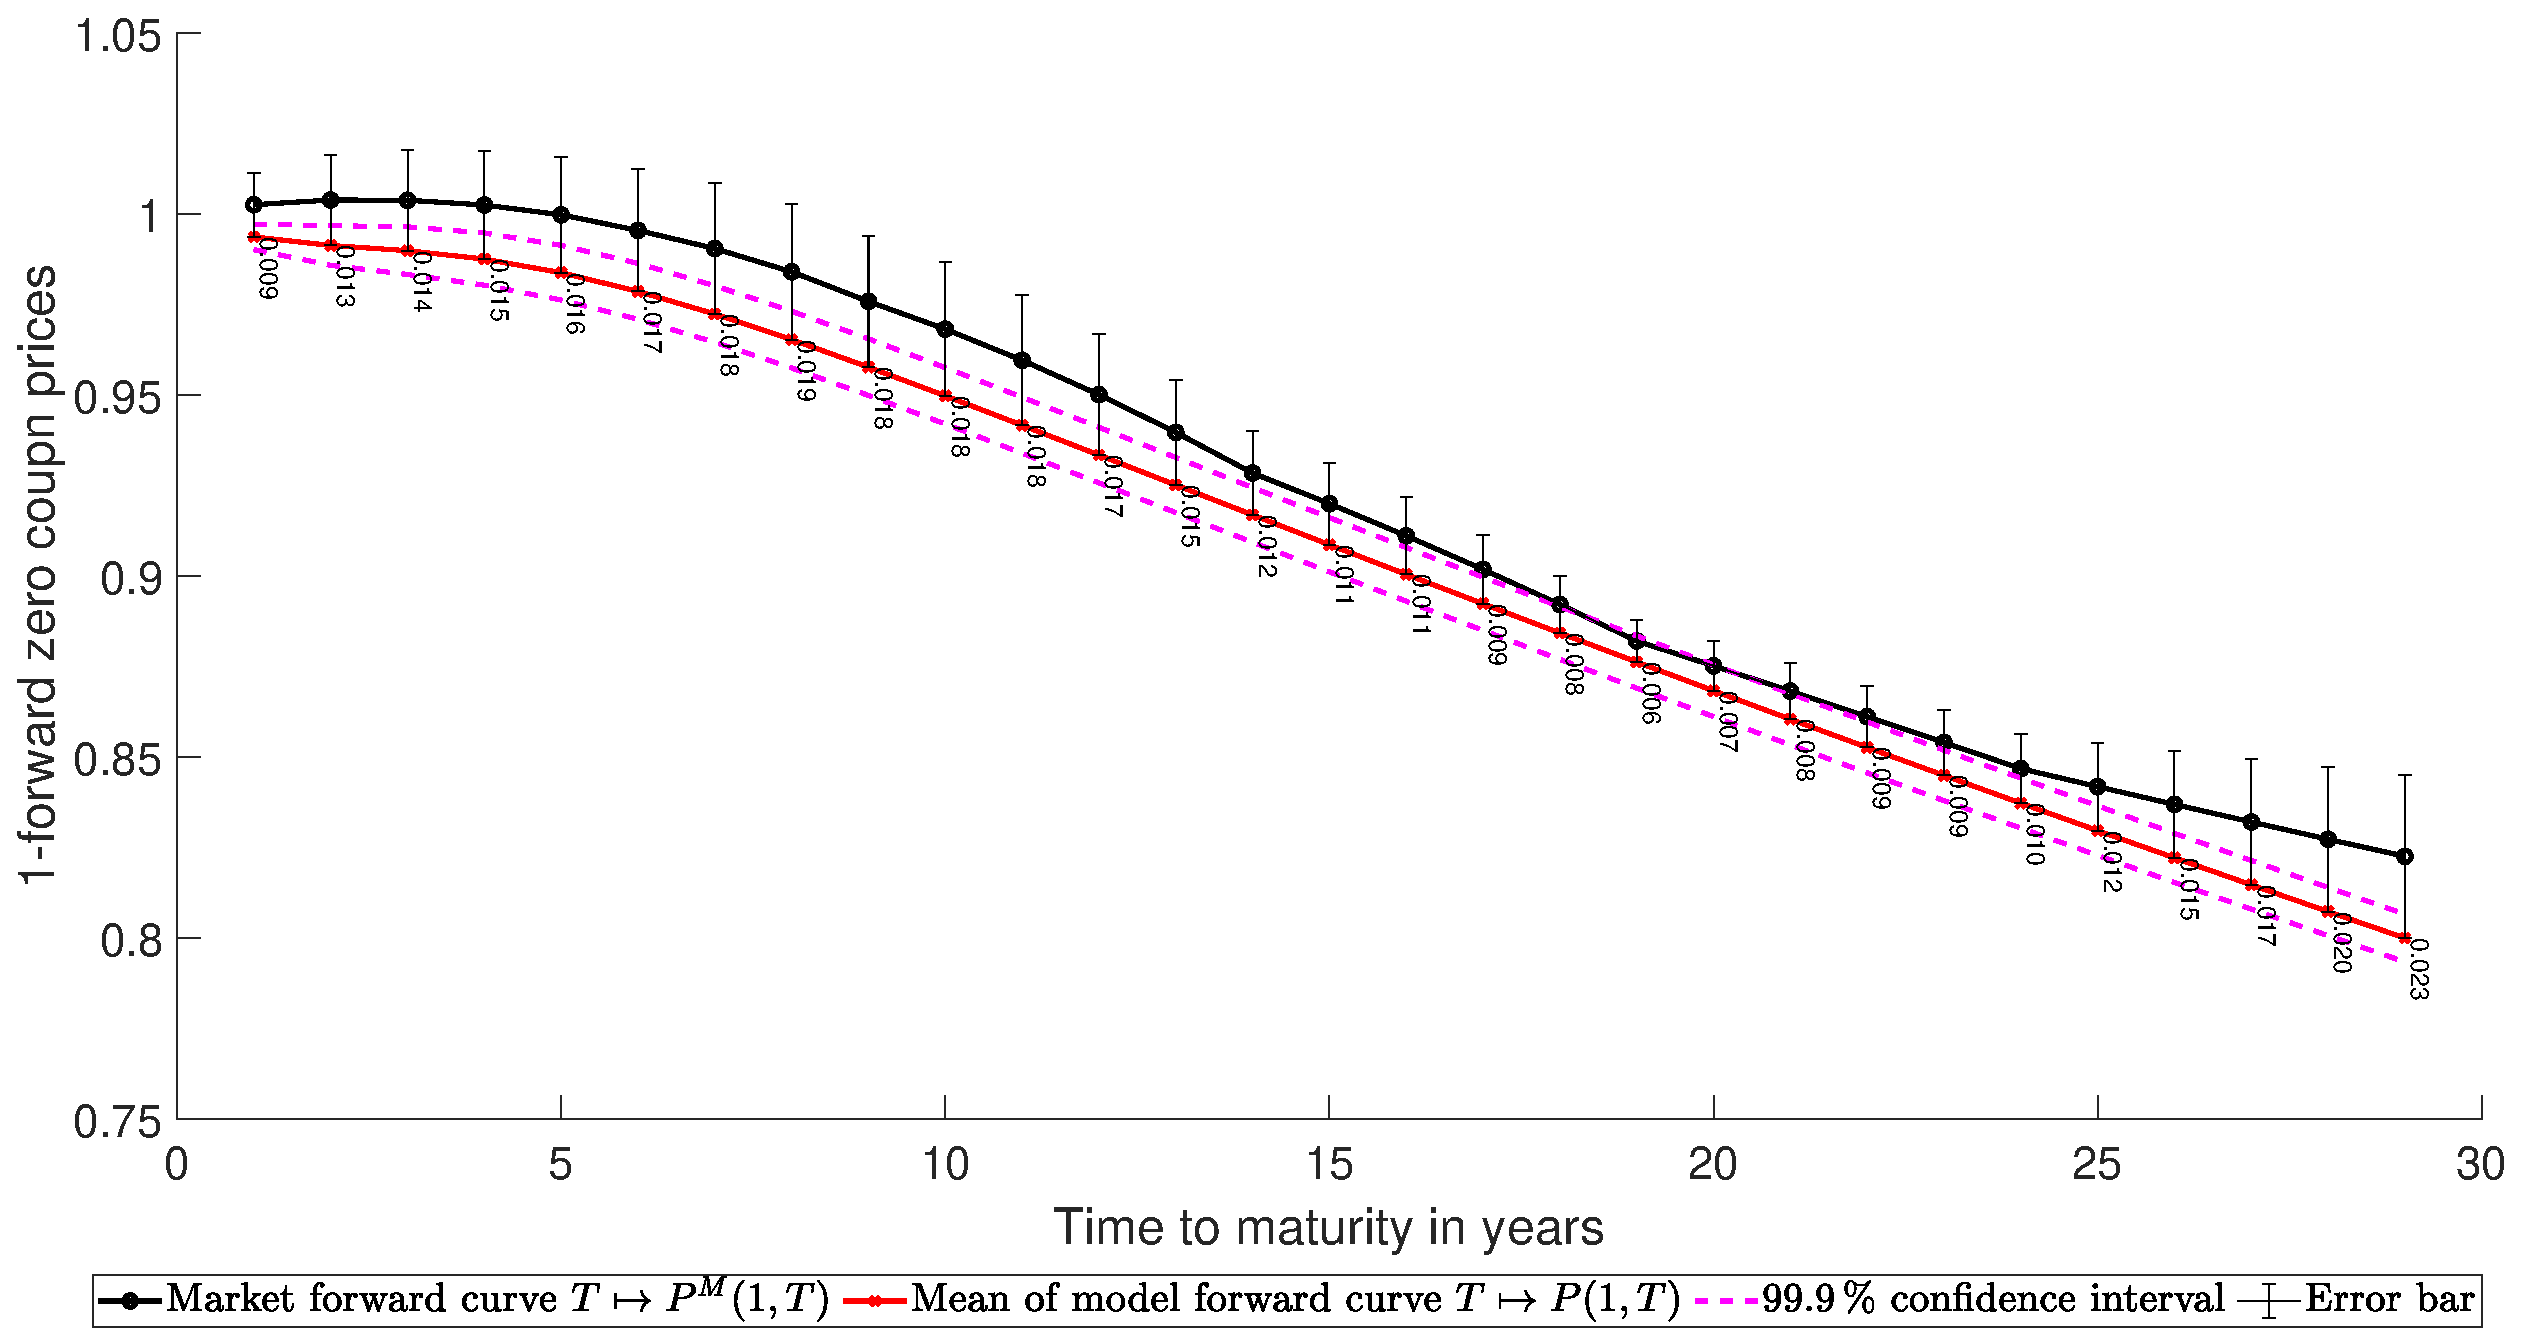
\includegraphics[width=.95\columnwidth]{Forward/F_A_1}
\end{landscape}
\begin{landscape}
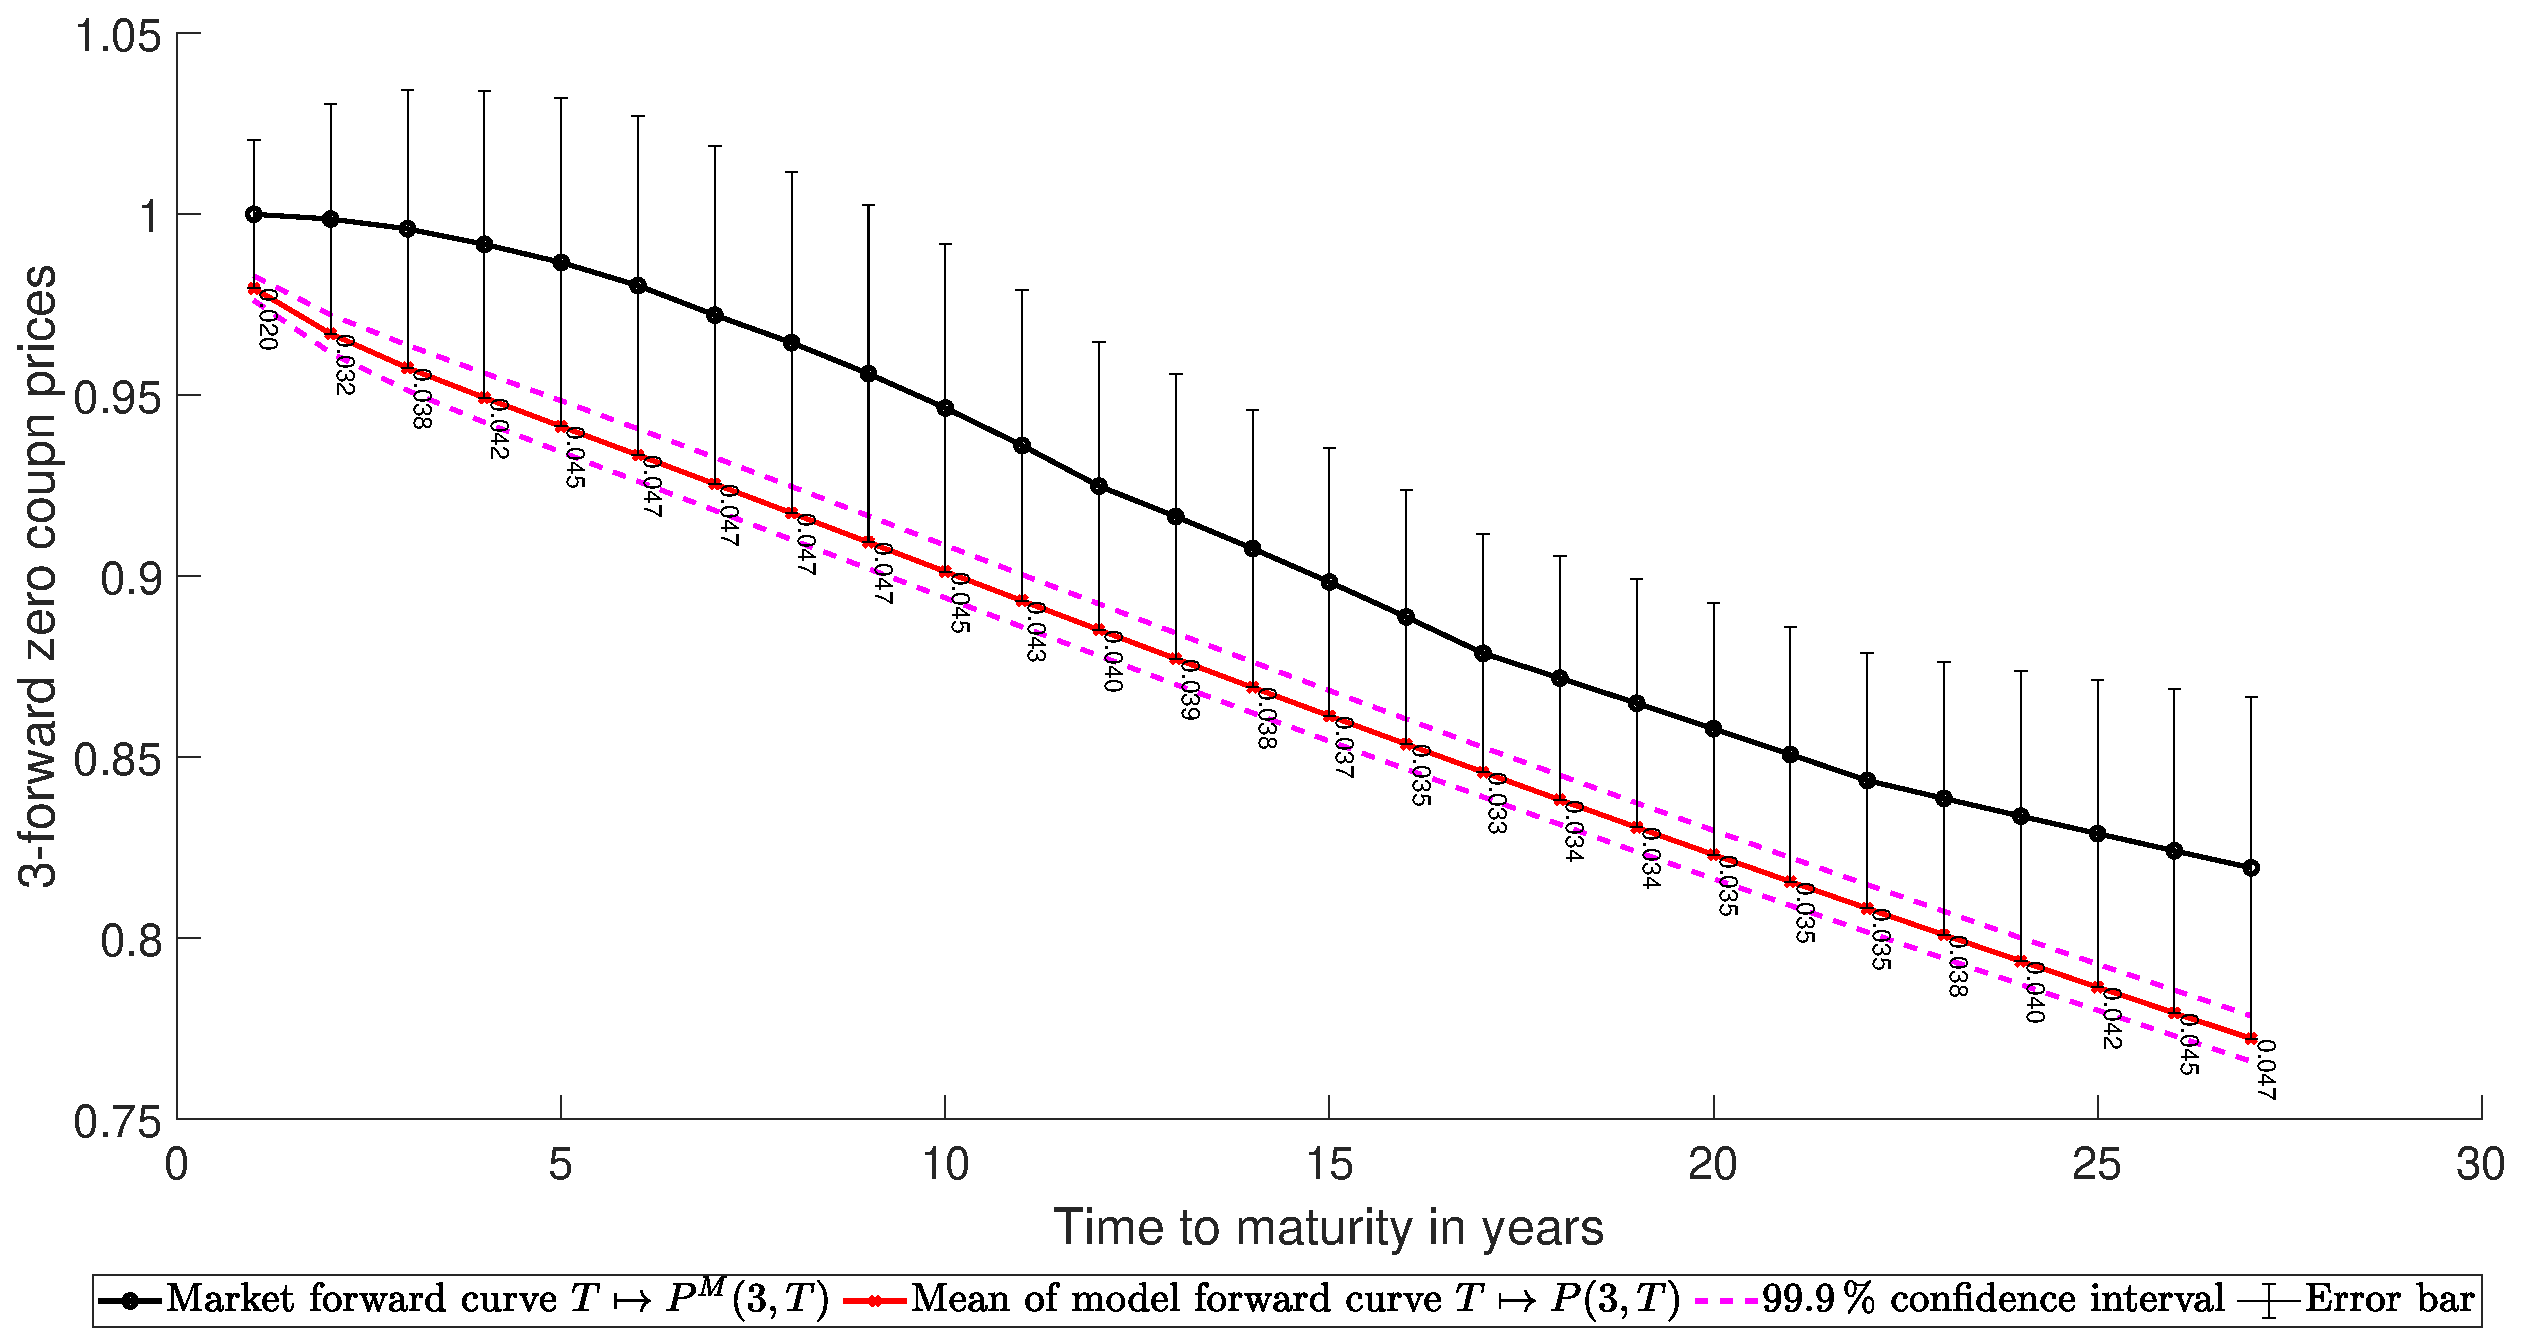
\includegraphics[width=.95\columnwidth]{Forward/F_A_2}
\end{landscape}
\begin{landscape}
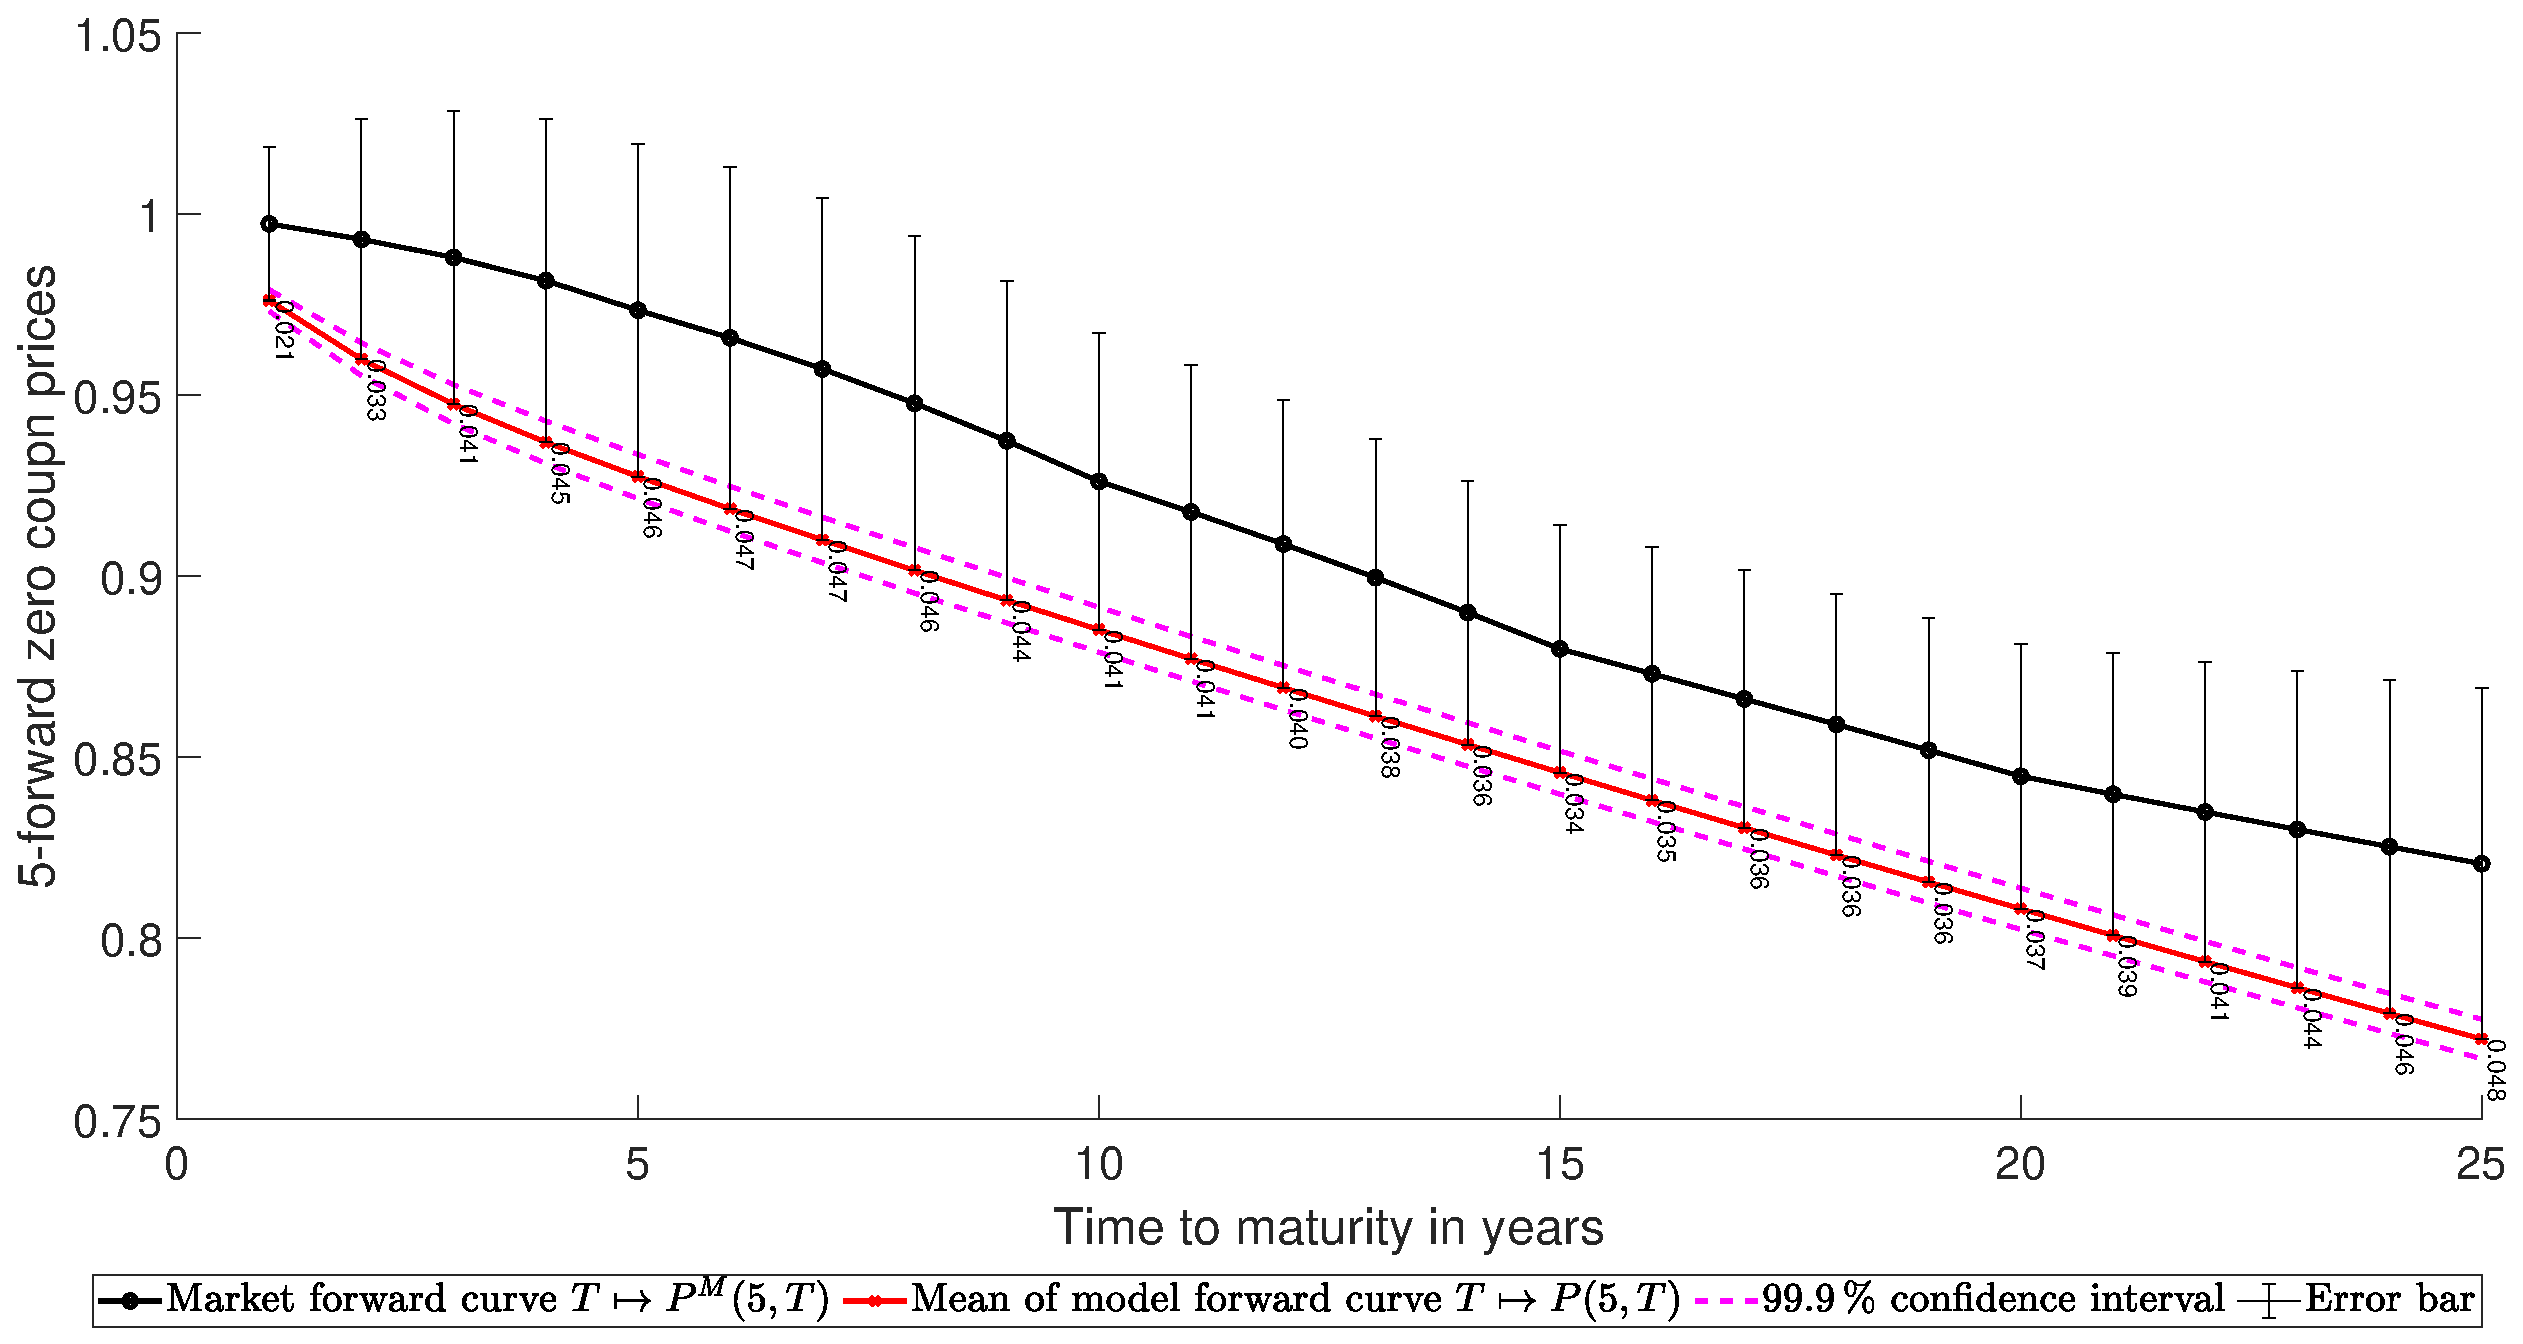
\includegraphics[width=.95\columnwidth]{Forward/F_A_3}
\end{landscape}

\subsection{Plots of Discount Factor}
	\begin{landscape}
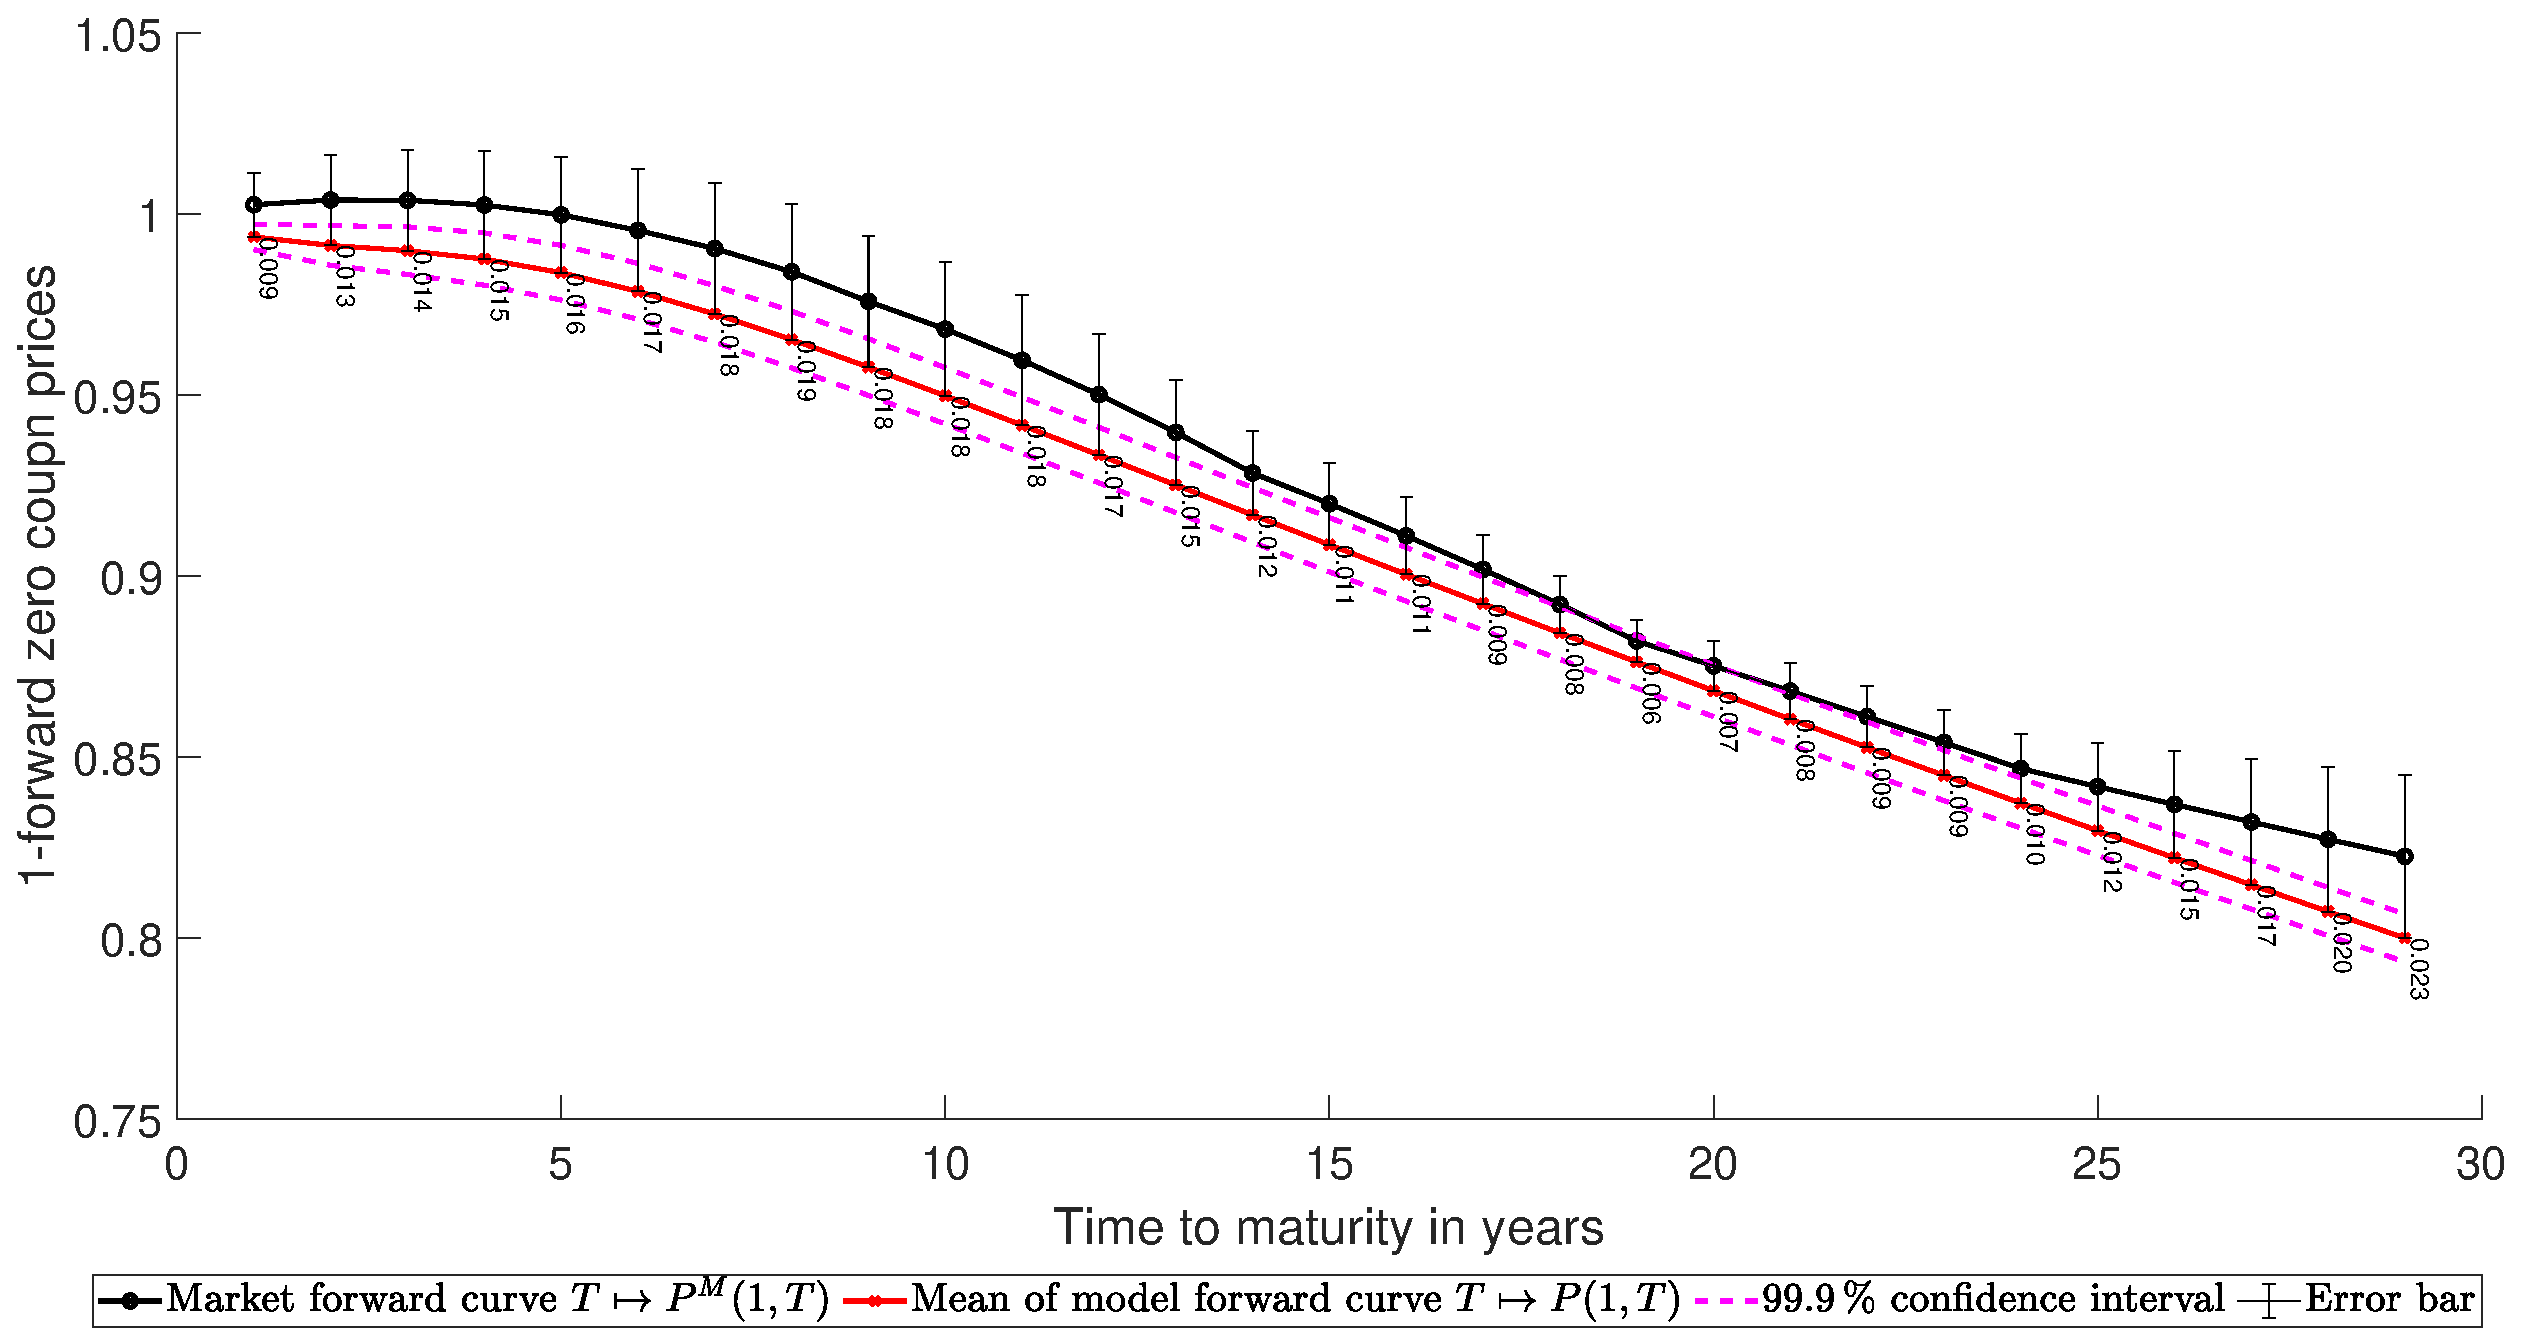
\includegraphics[width=.95\columnwidth]{Forward/F_A_1}
\end{landscape}
\begin{landscape}
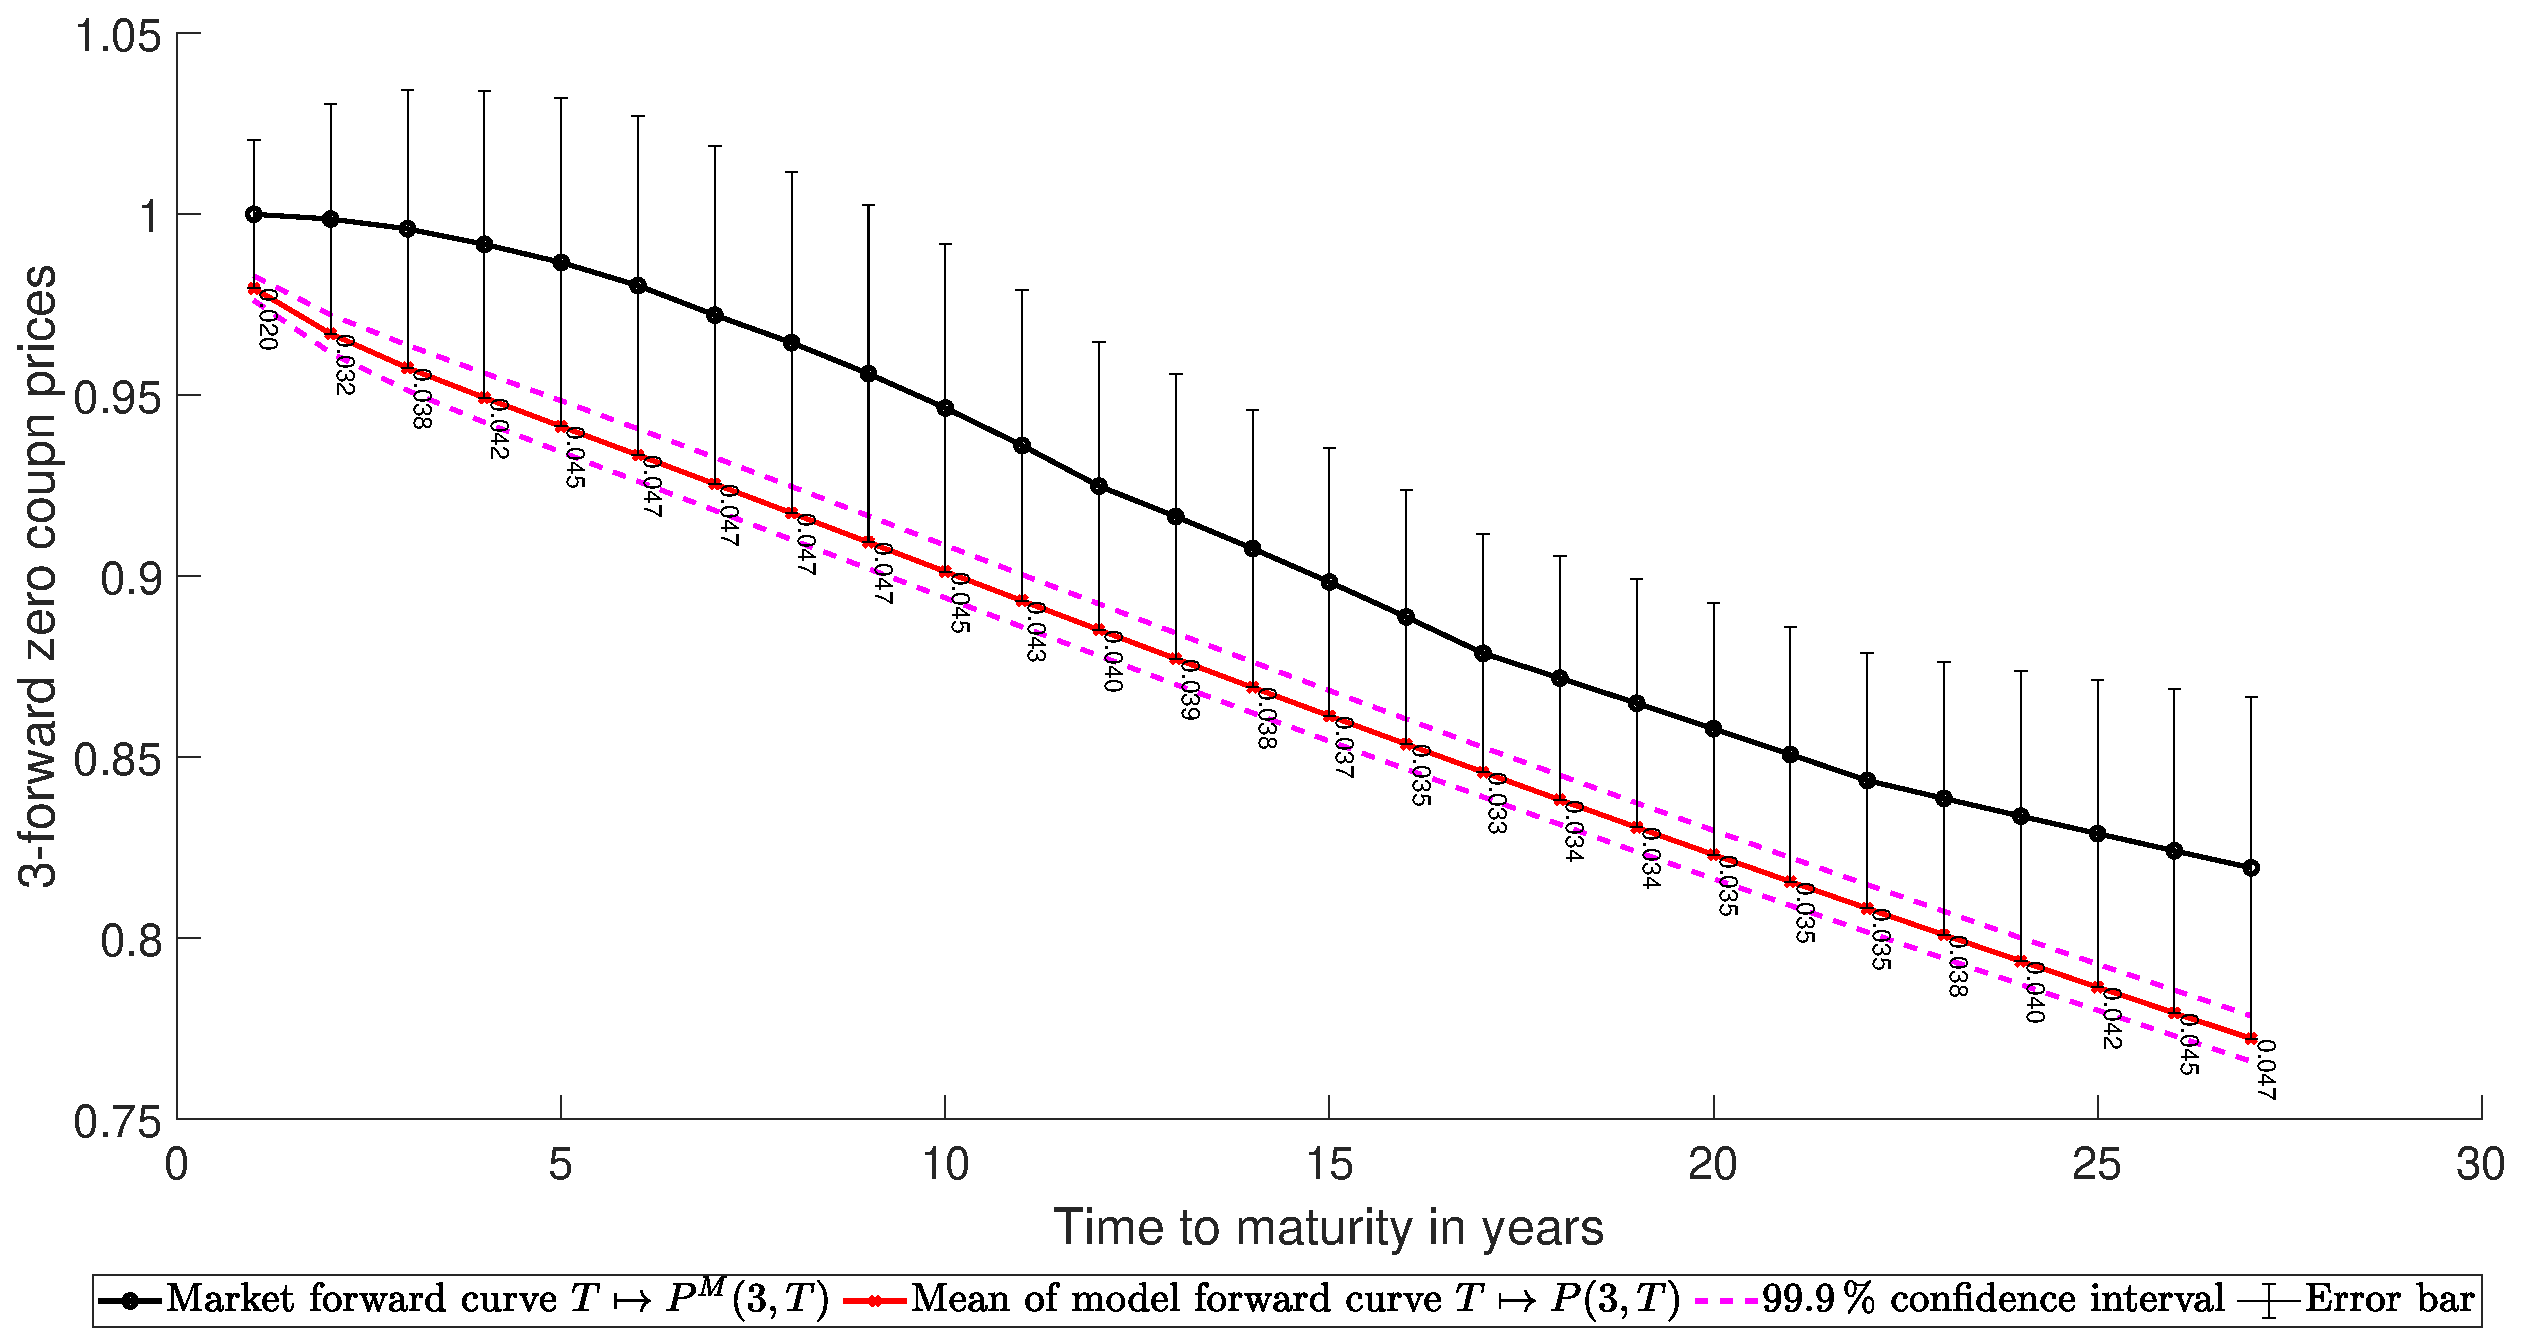
\includegraphics[width=.95\columnwidth]{Forward/F_A_2}
\end{landscape}
\begin{landscape}
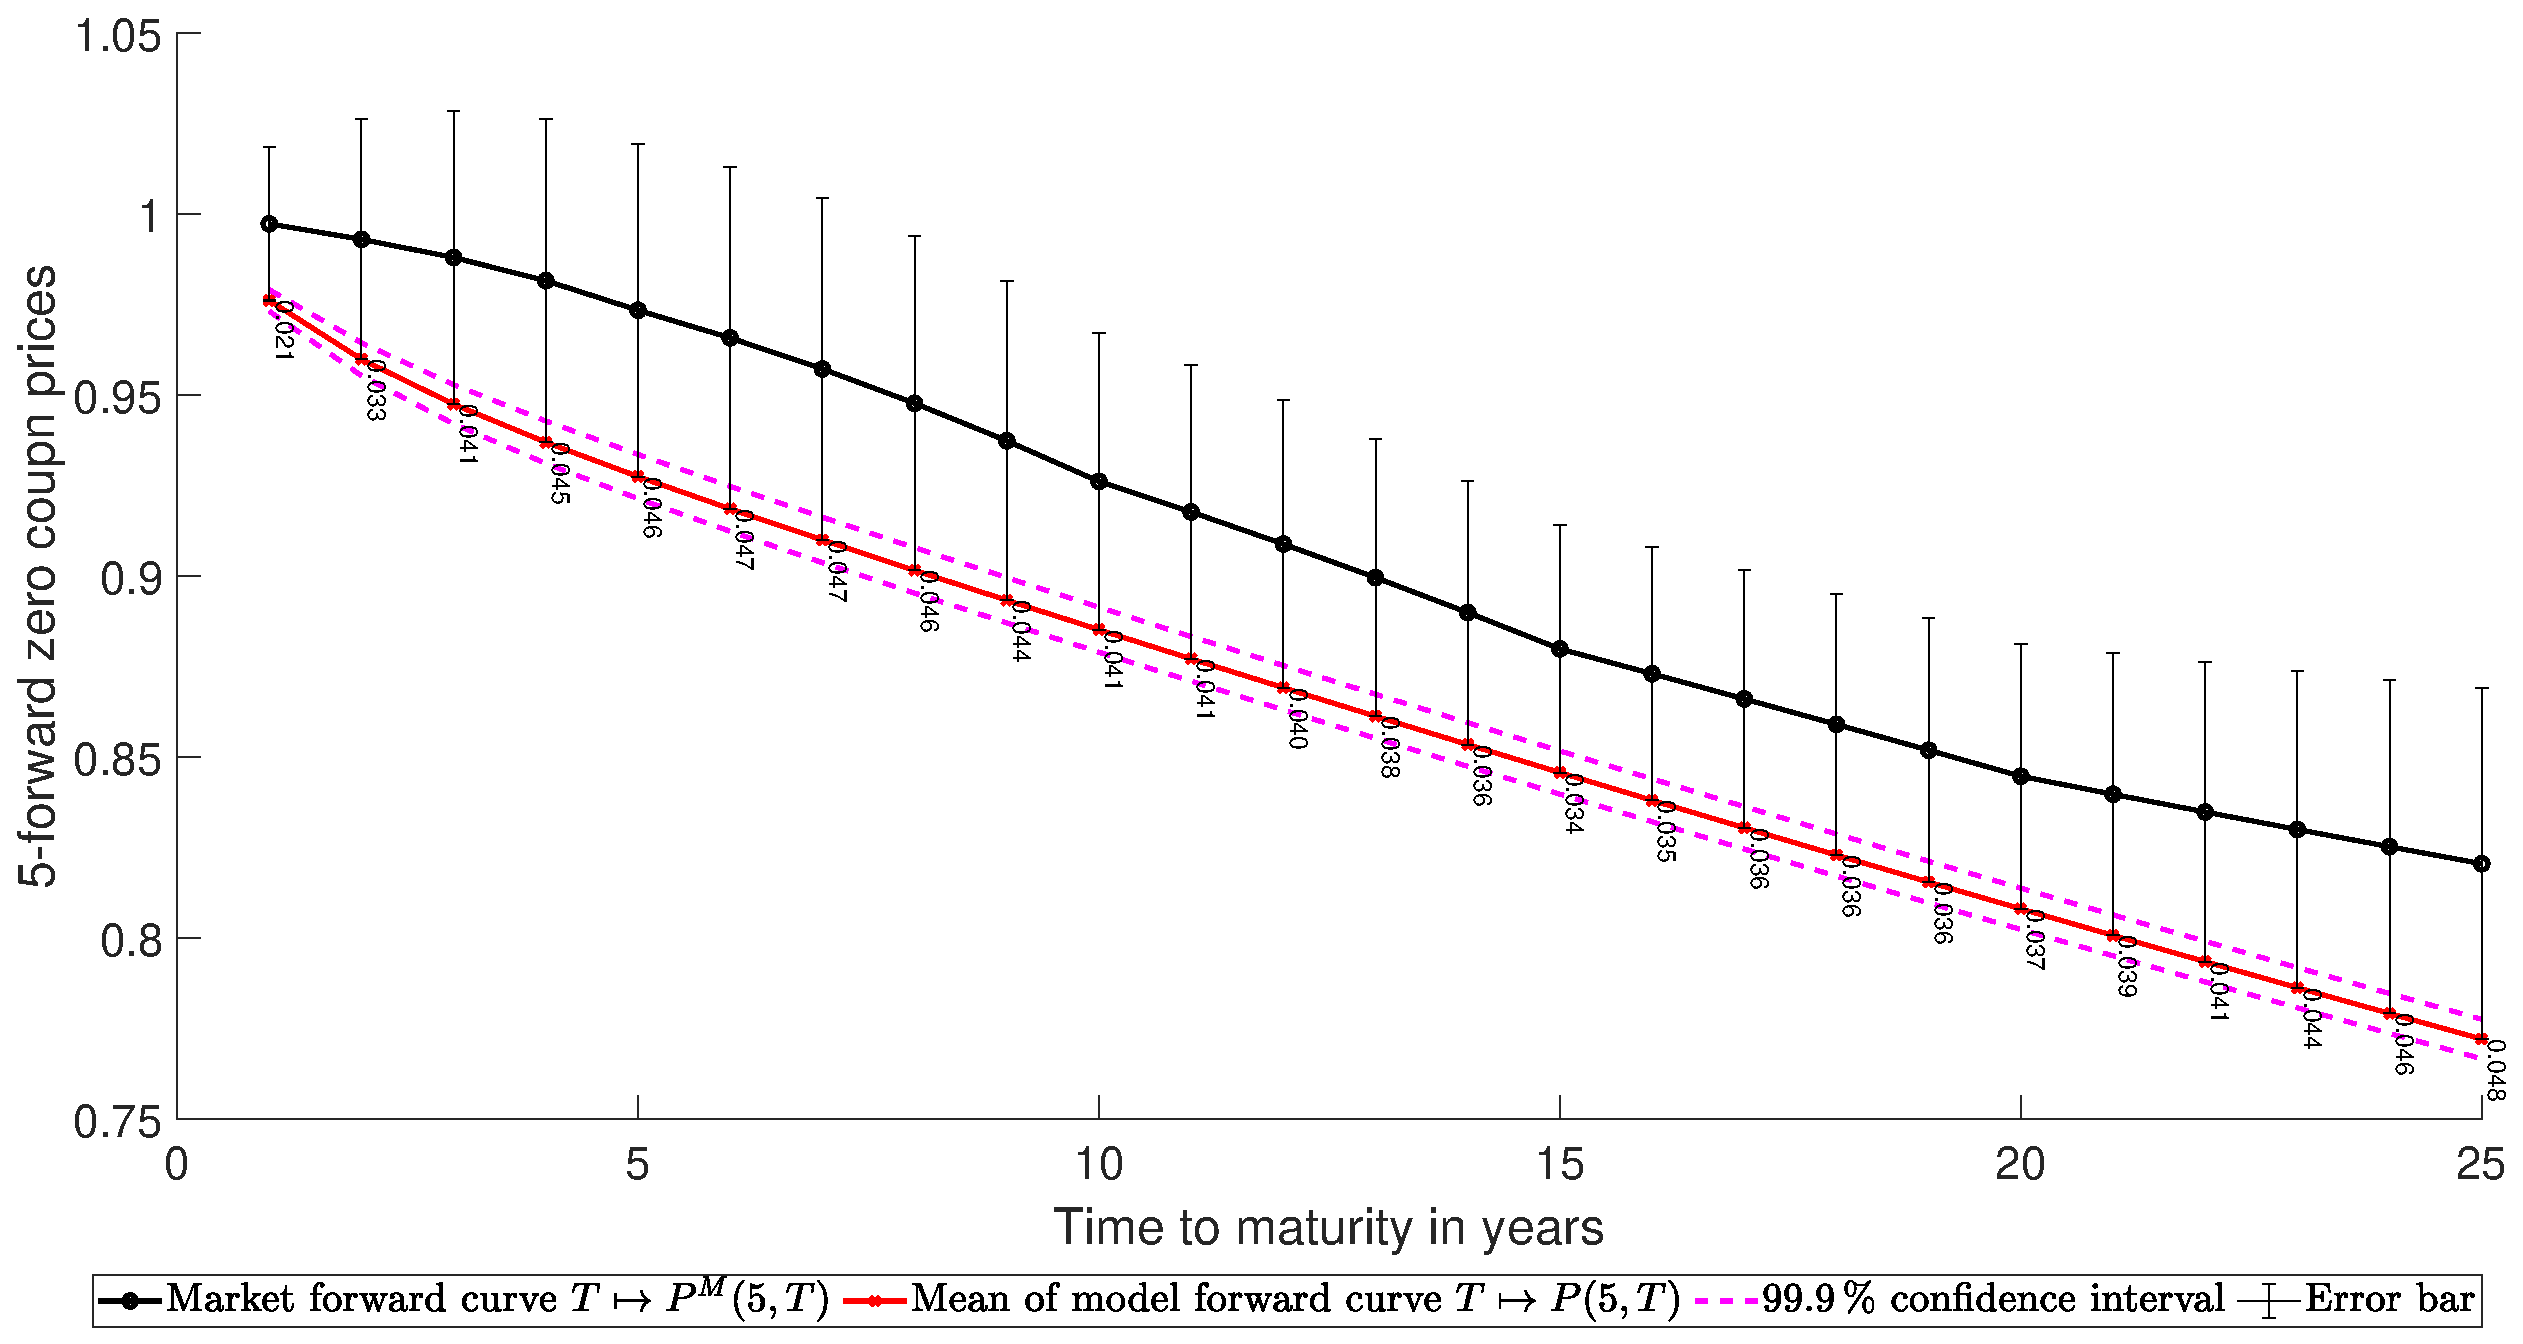
\includegraphics[width=.95\columnwidth]{Forward/F_A_3}
\end{landscape}

\subsection{Plots of Interest Rates}
	\begin{landscape}
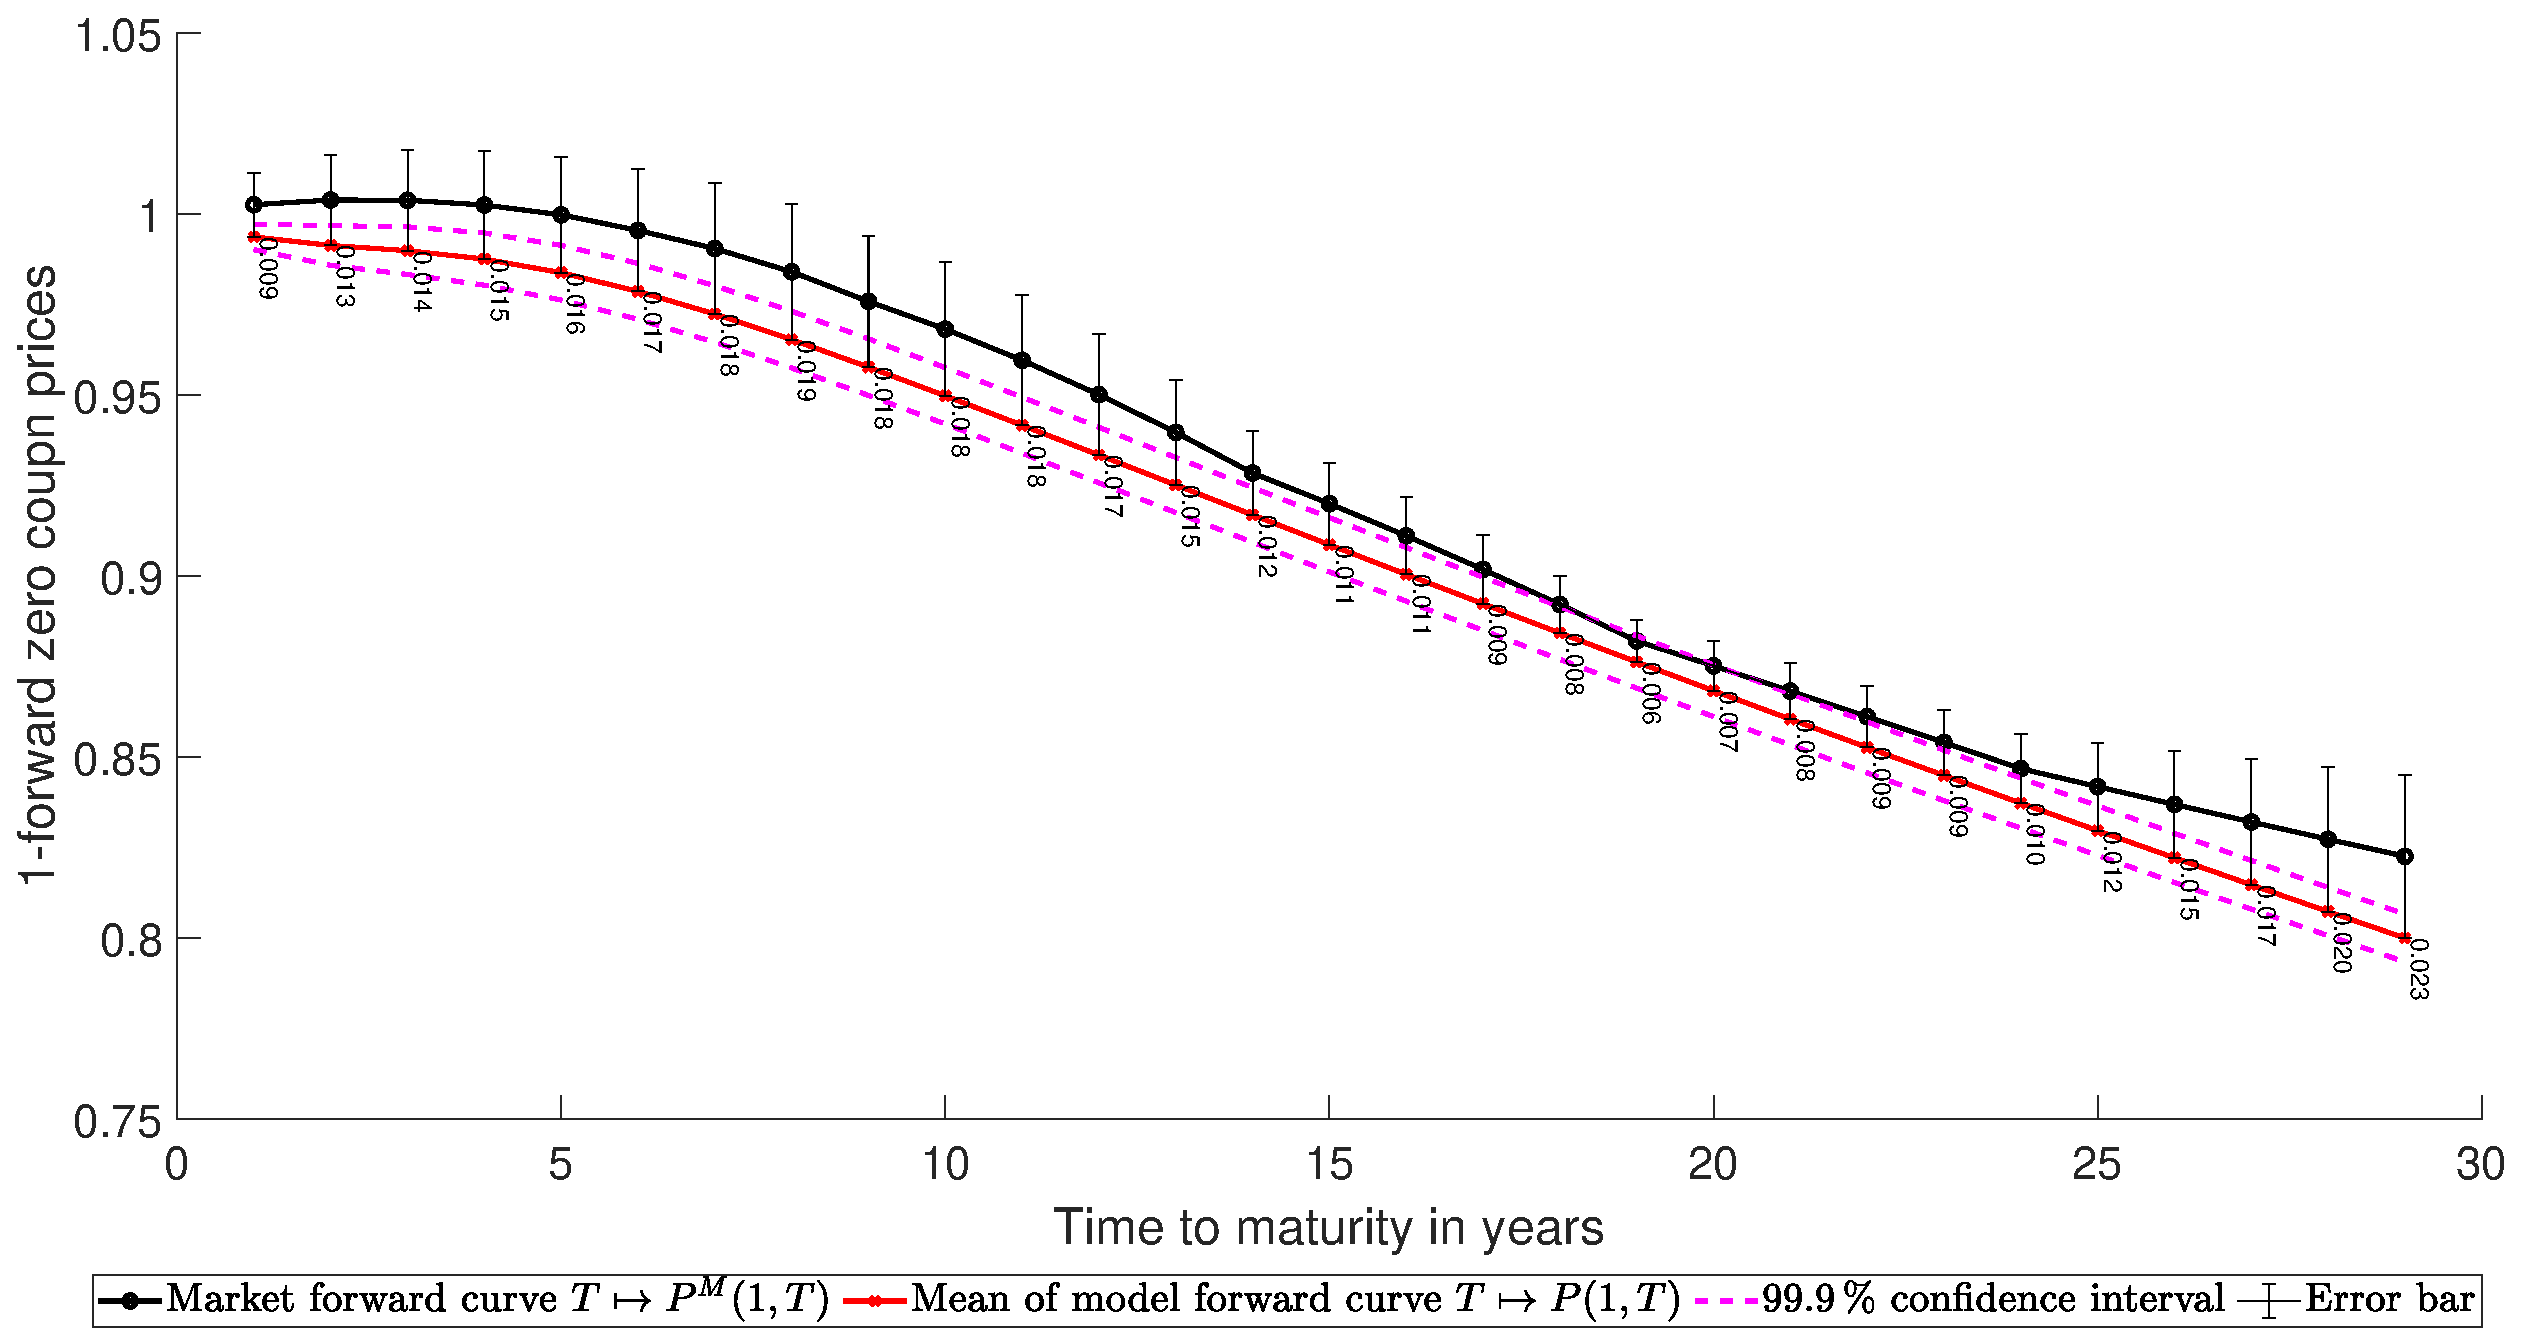
\includegraphics[width=.95\columnwidth]{Forward/F_A_1}
\end{landscape}
\begin{landscape}
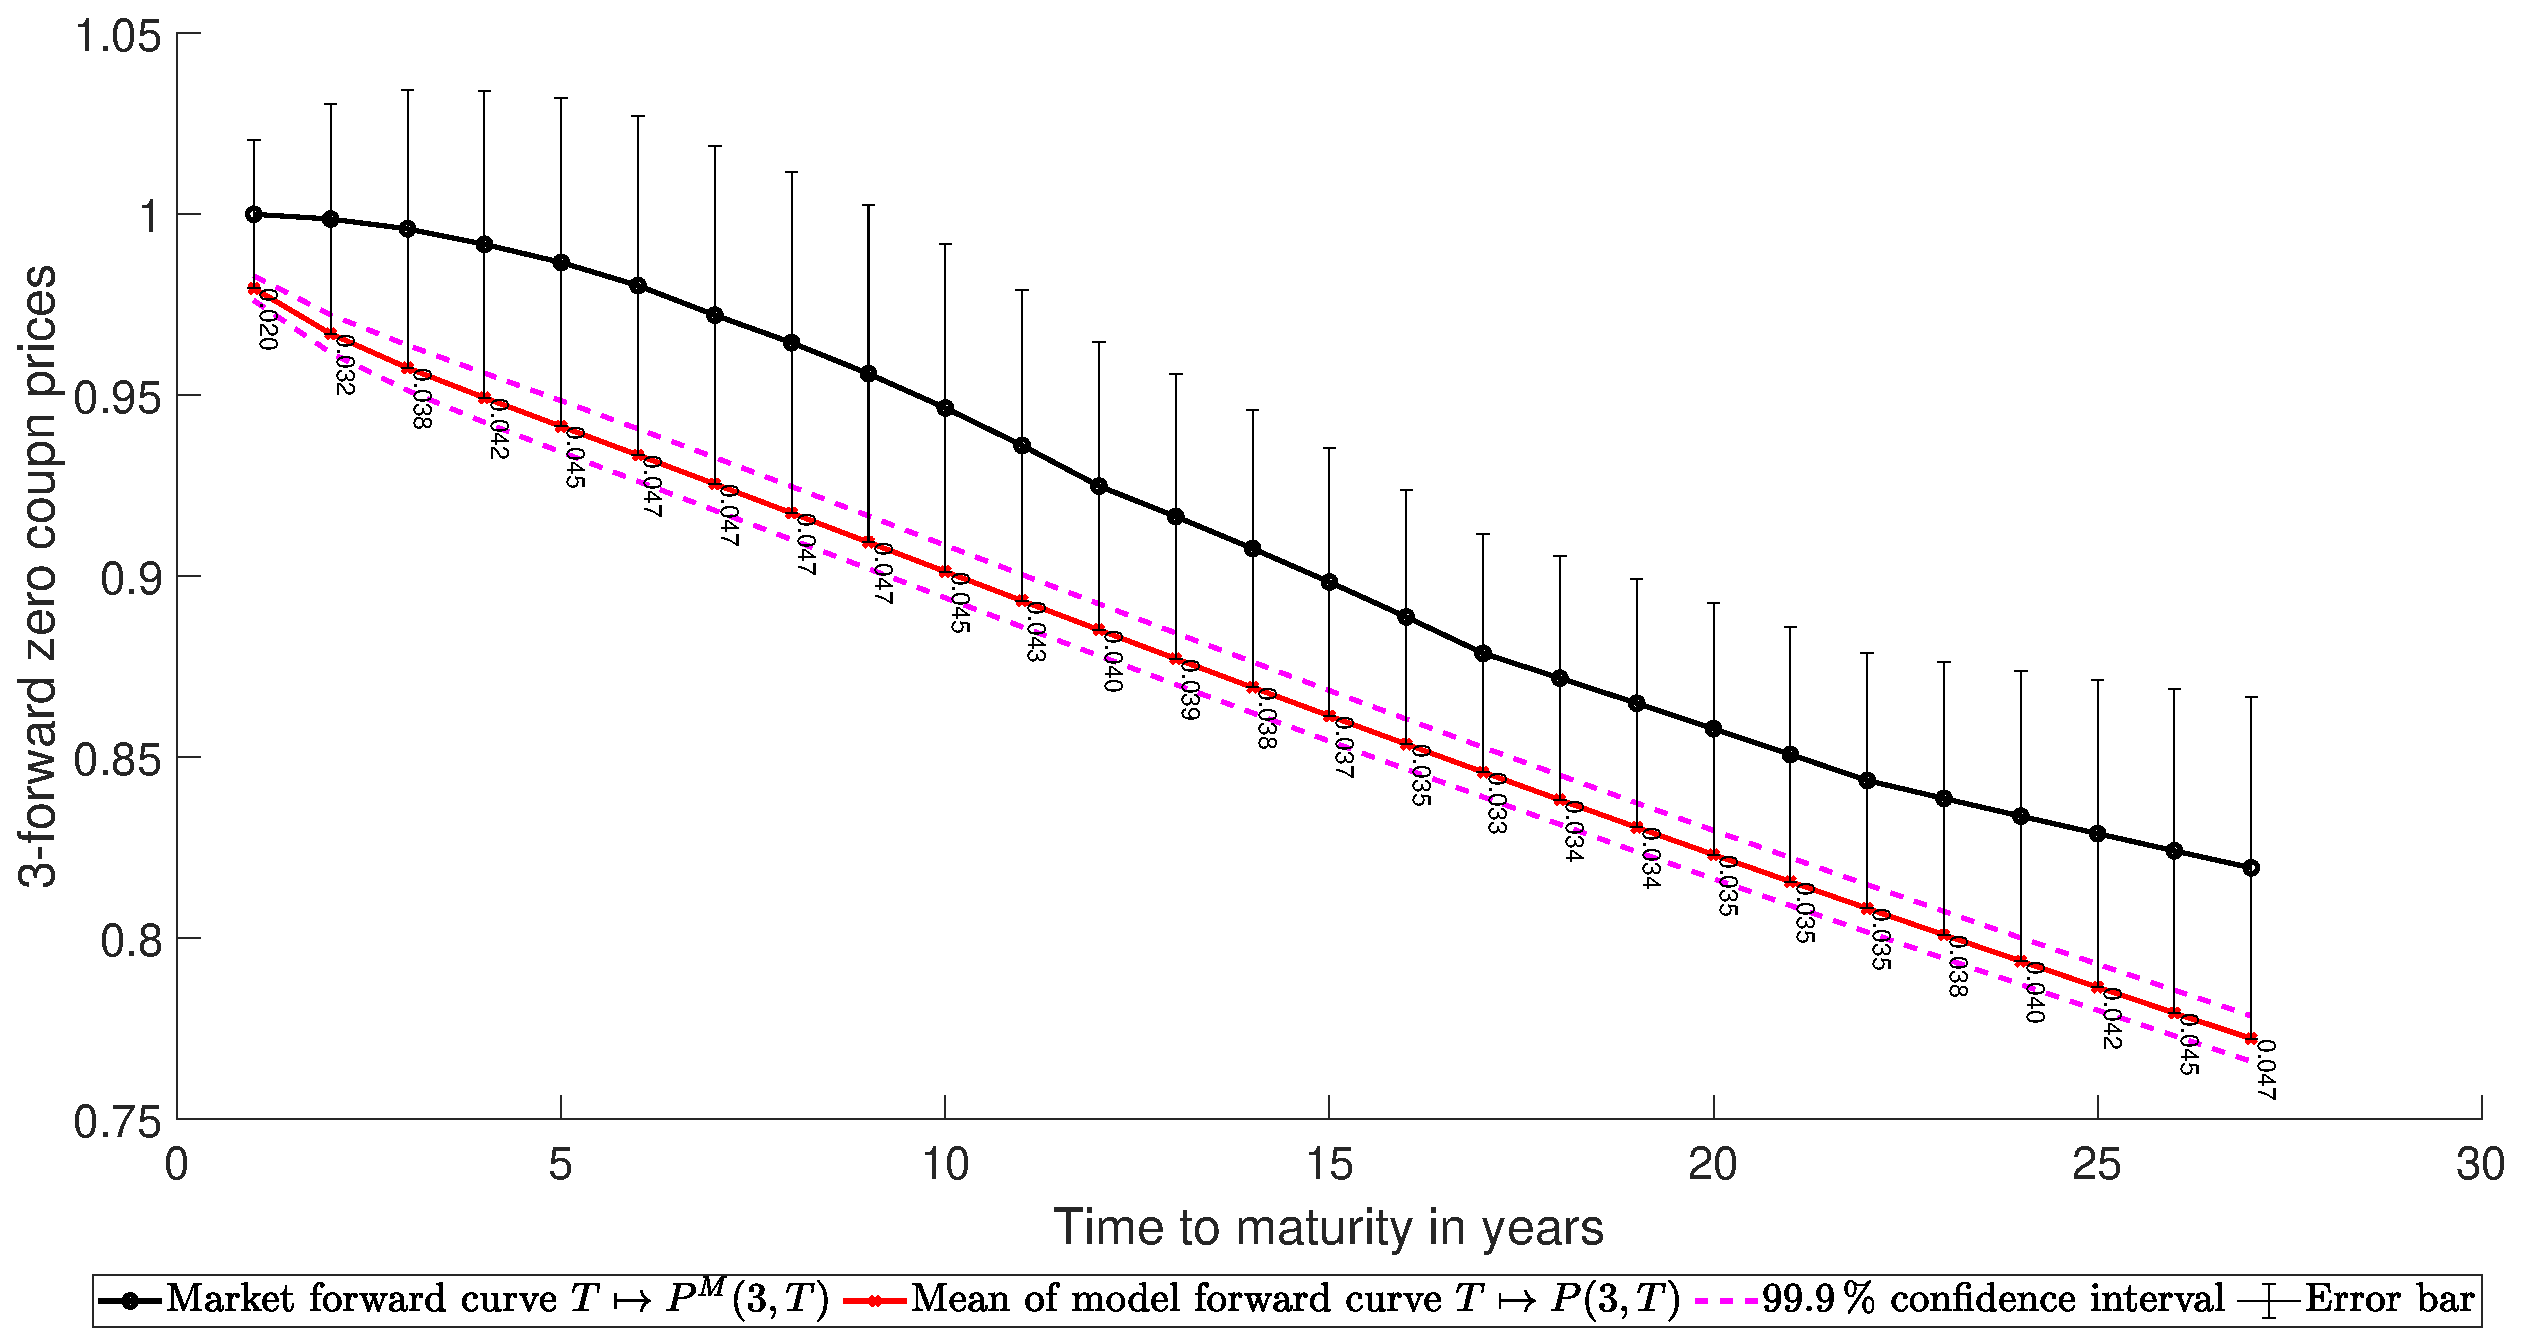
\includegraphics[width=.95\columnwidth]{Forward/F_A_2}
\end{landscape}
\begin{landscape}
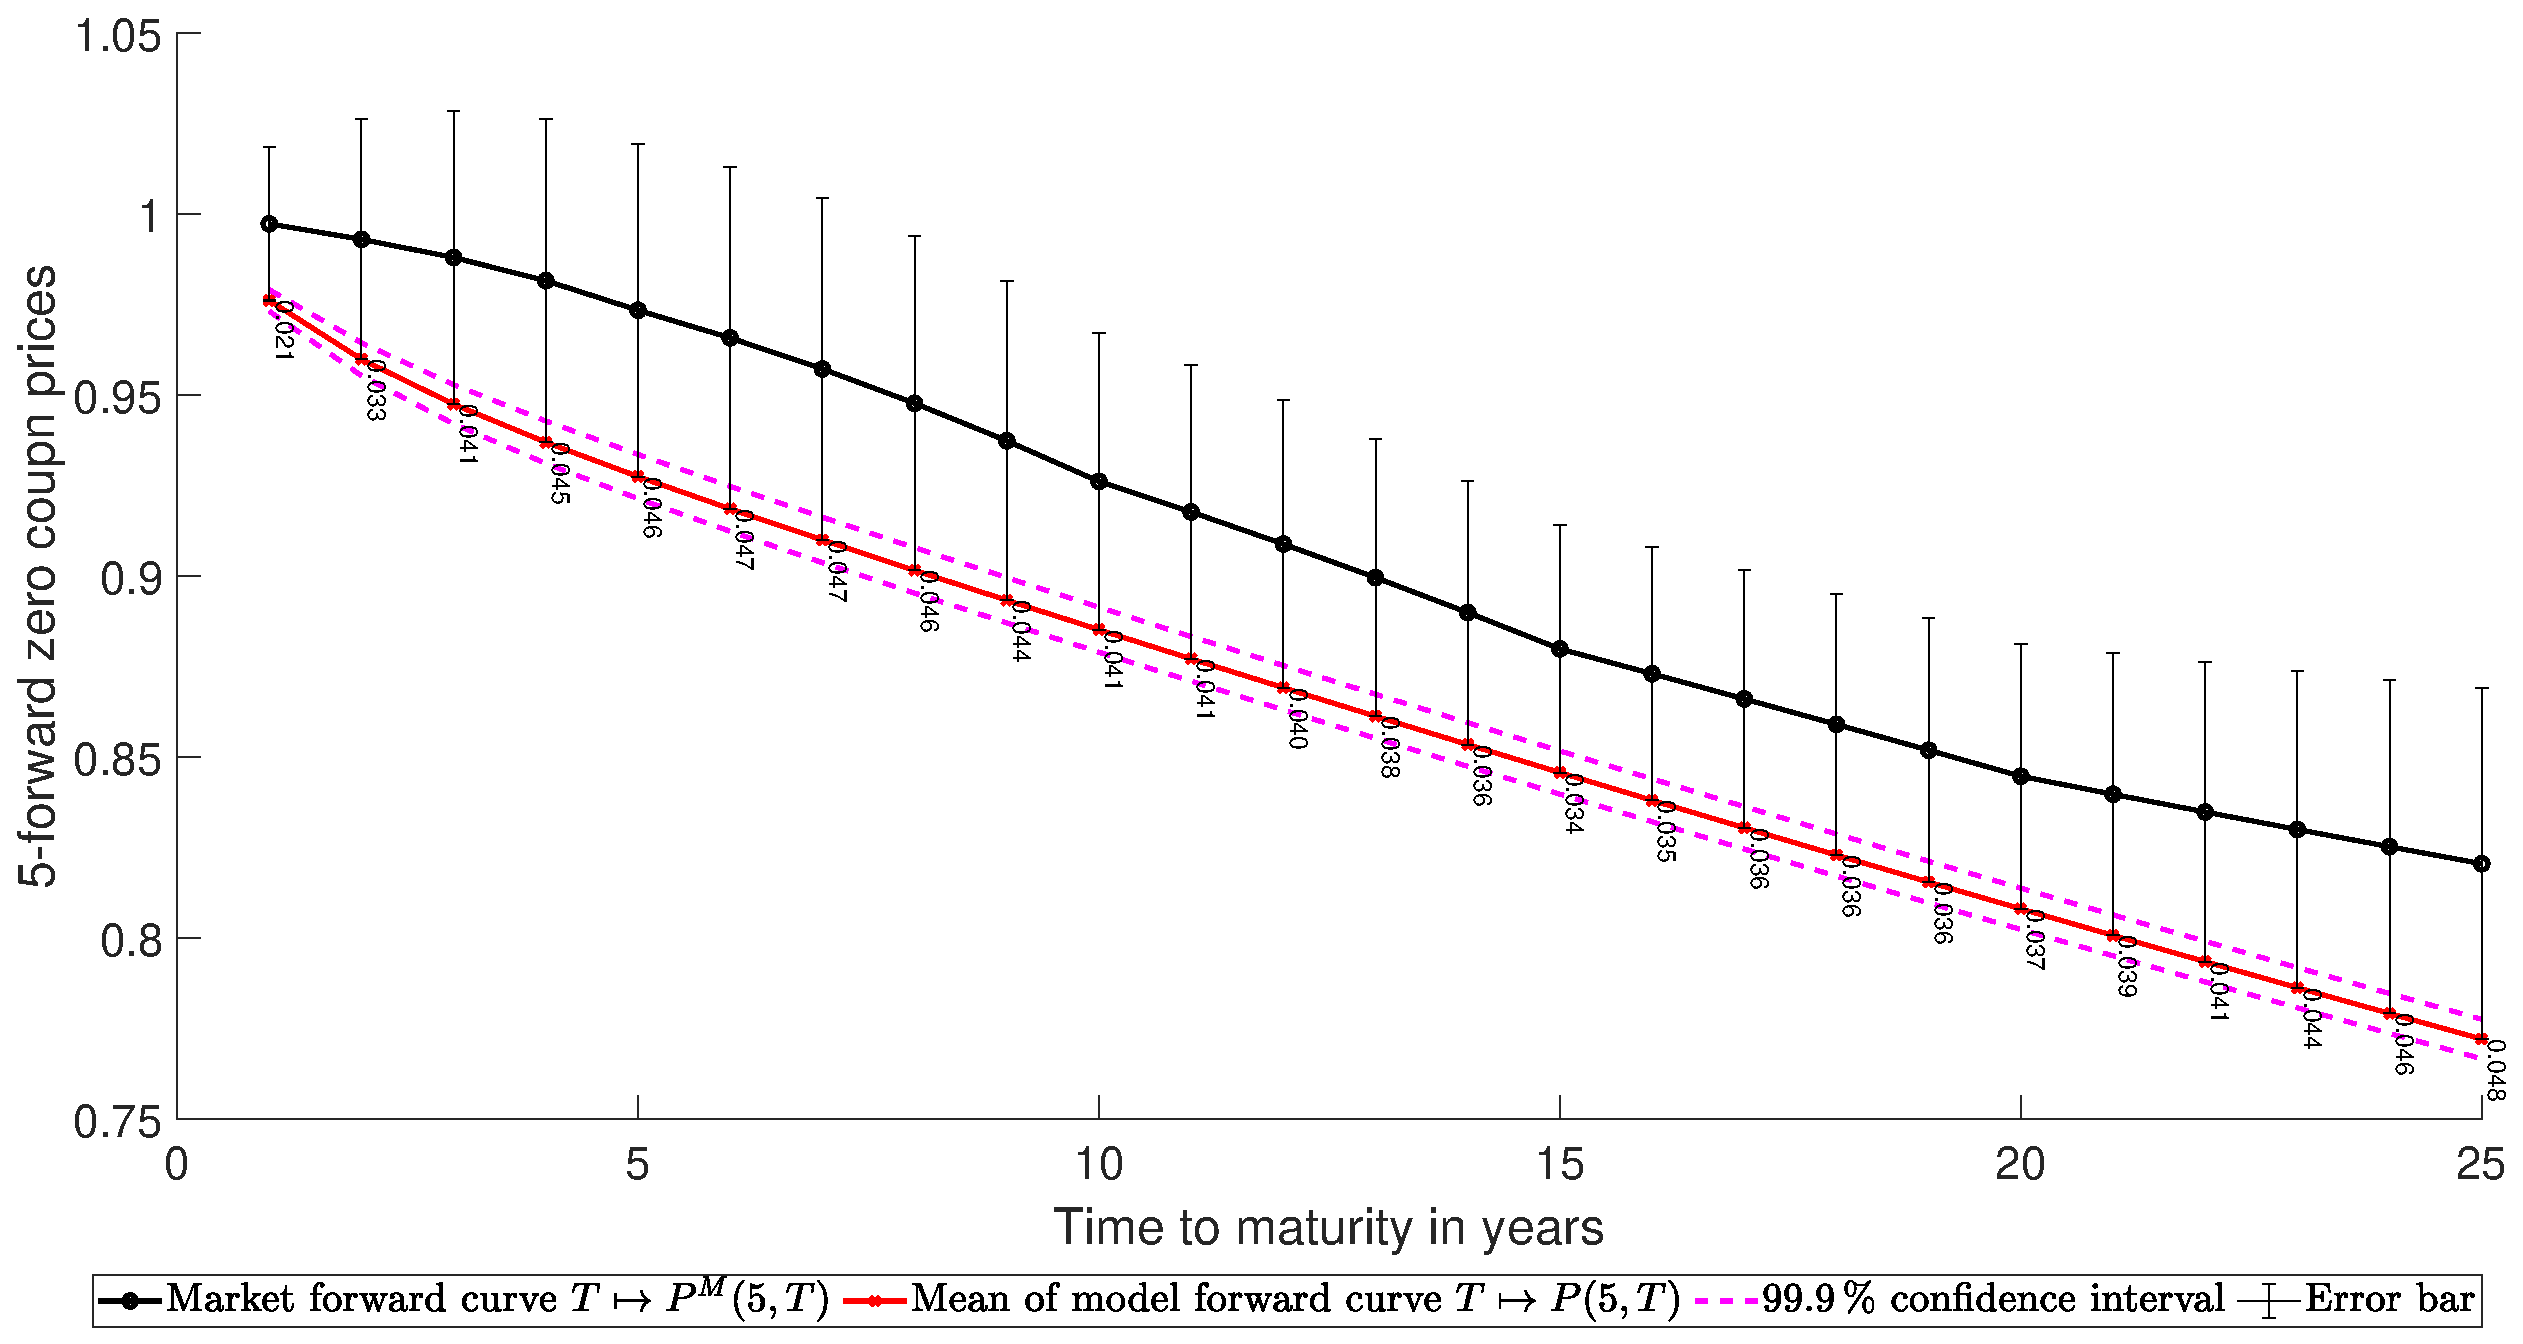
\includegraphics[width=.95\columnwidth]{Forward/F_A_3}
\end{landscape}

\subsection{Plots of theoretical Mean and Variance}
	\begin{landscape}
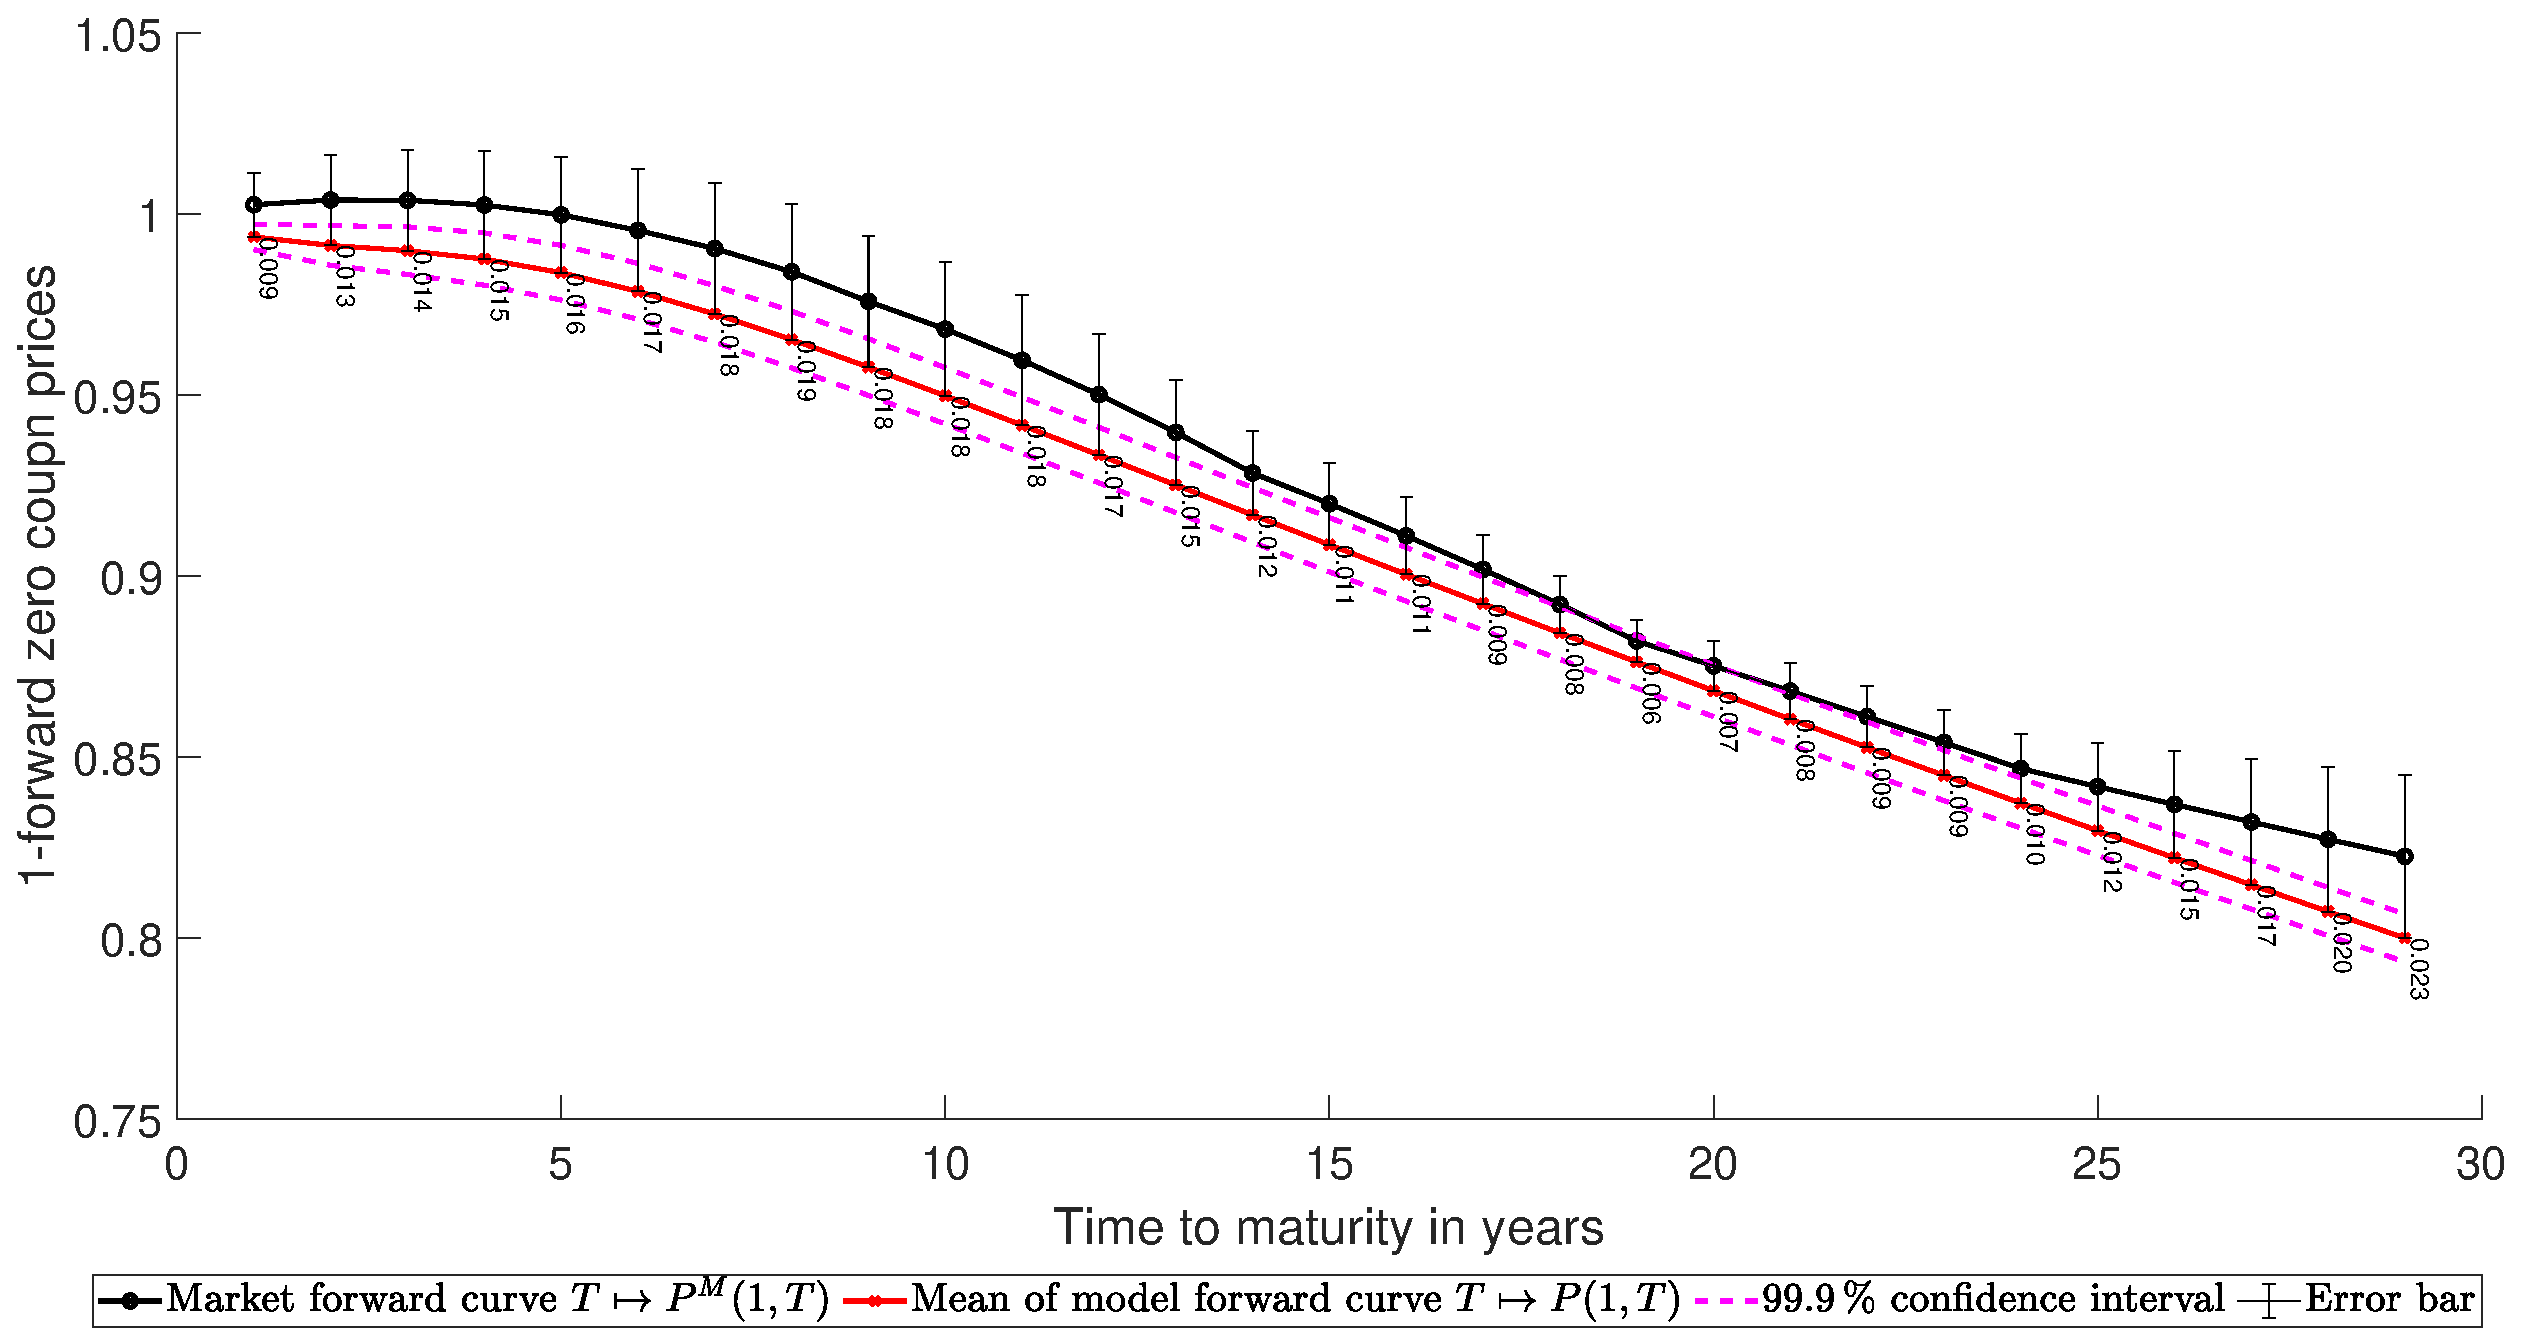
\includegraphics[width=.95\columnwidth]{Forward/F_A_1}
\end{landscape}
\begin{landscape}
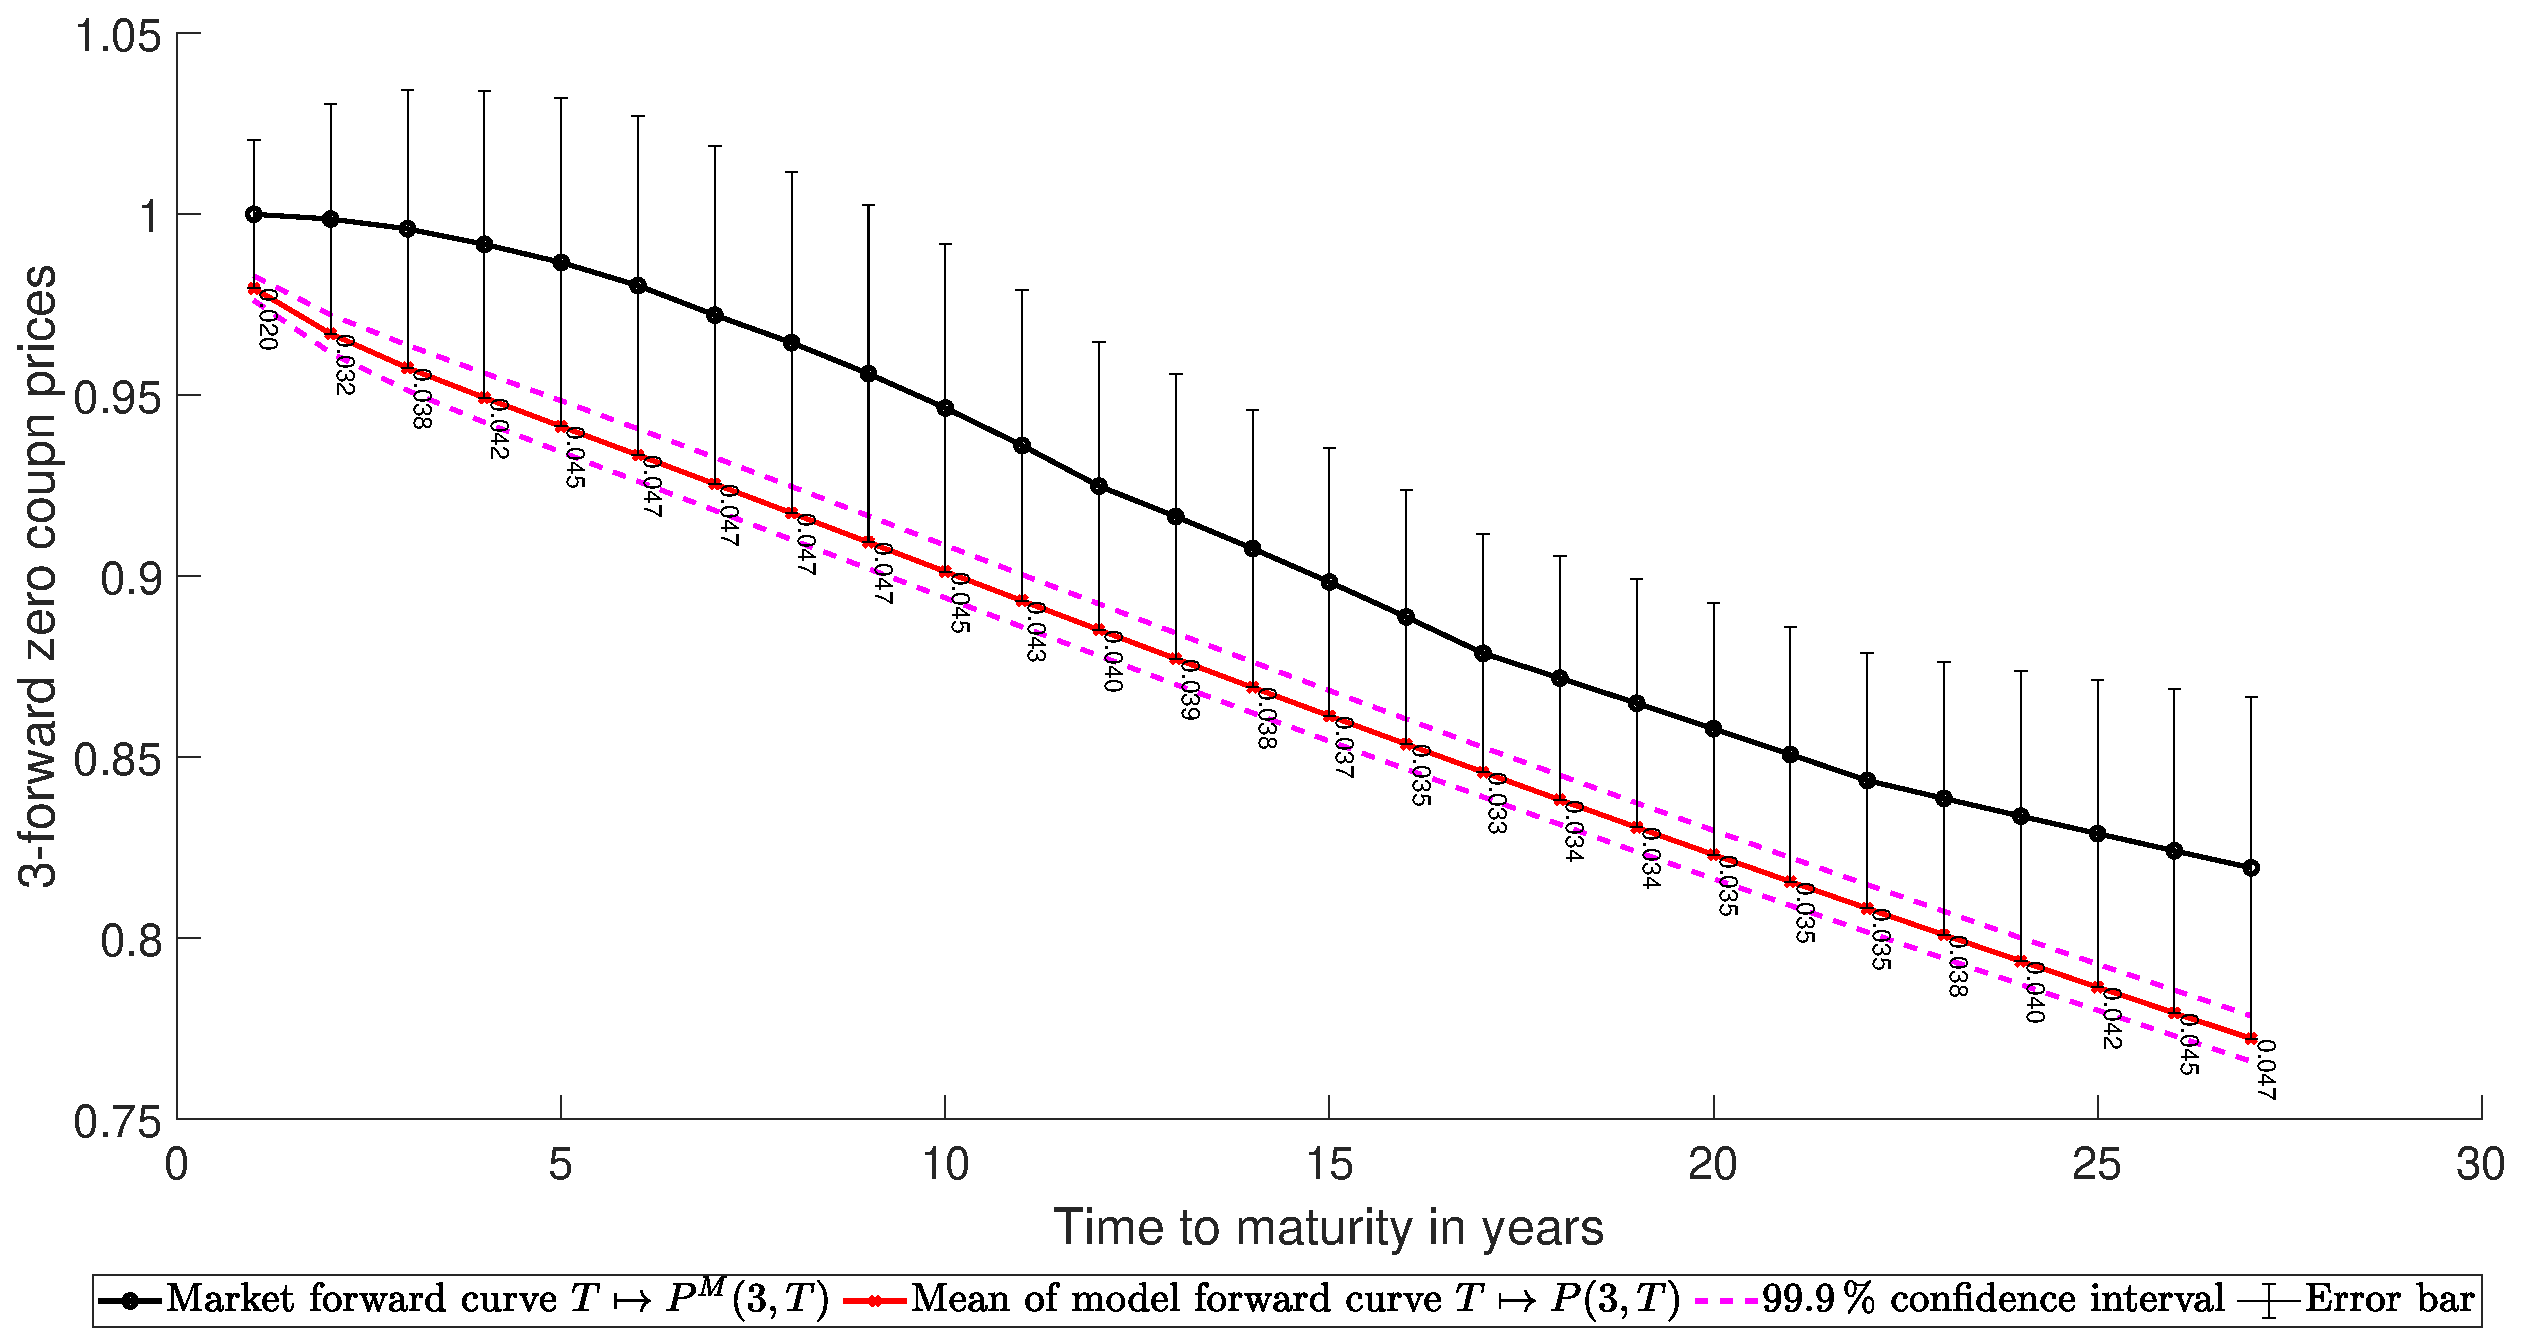
\includegraphics[width=.95\columnwidth]{Forward/F_A_2}
\end{landscape}
\begin{landscape}
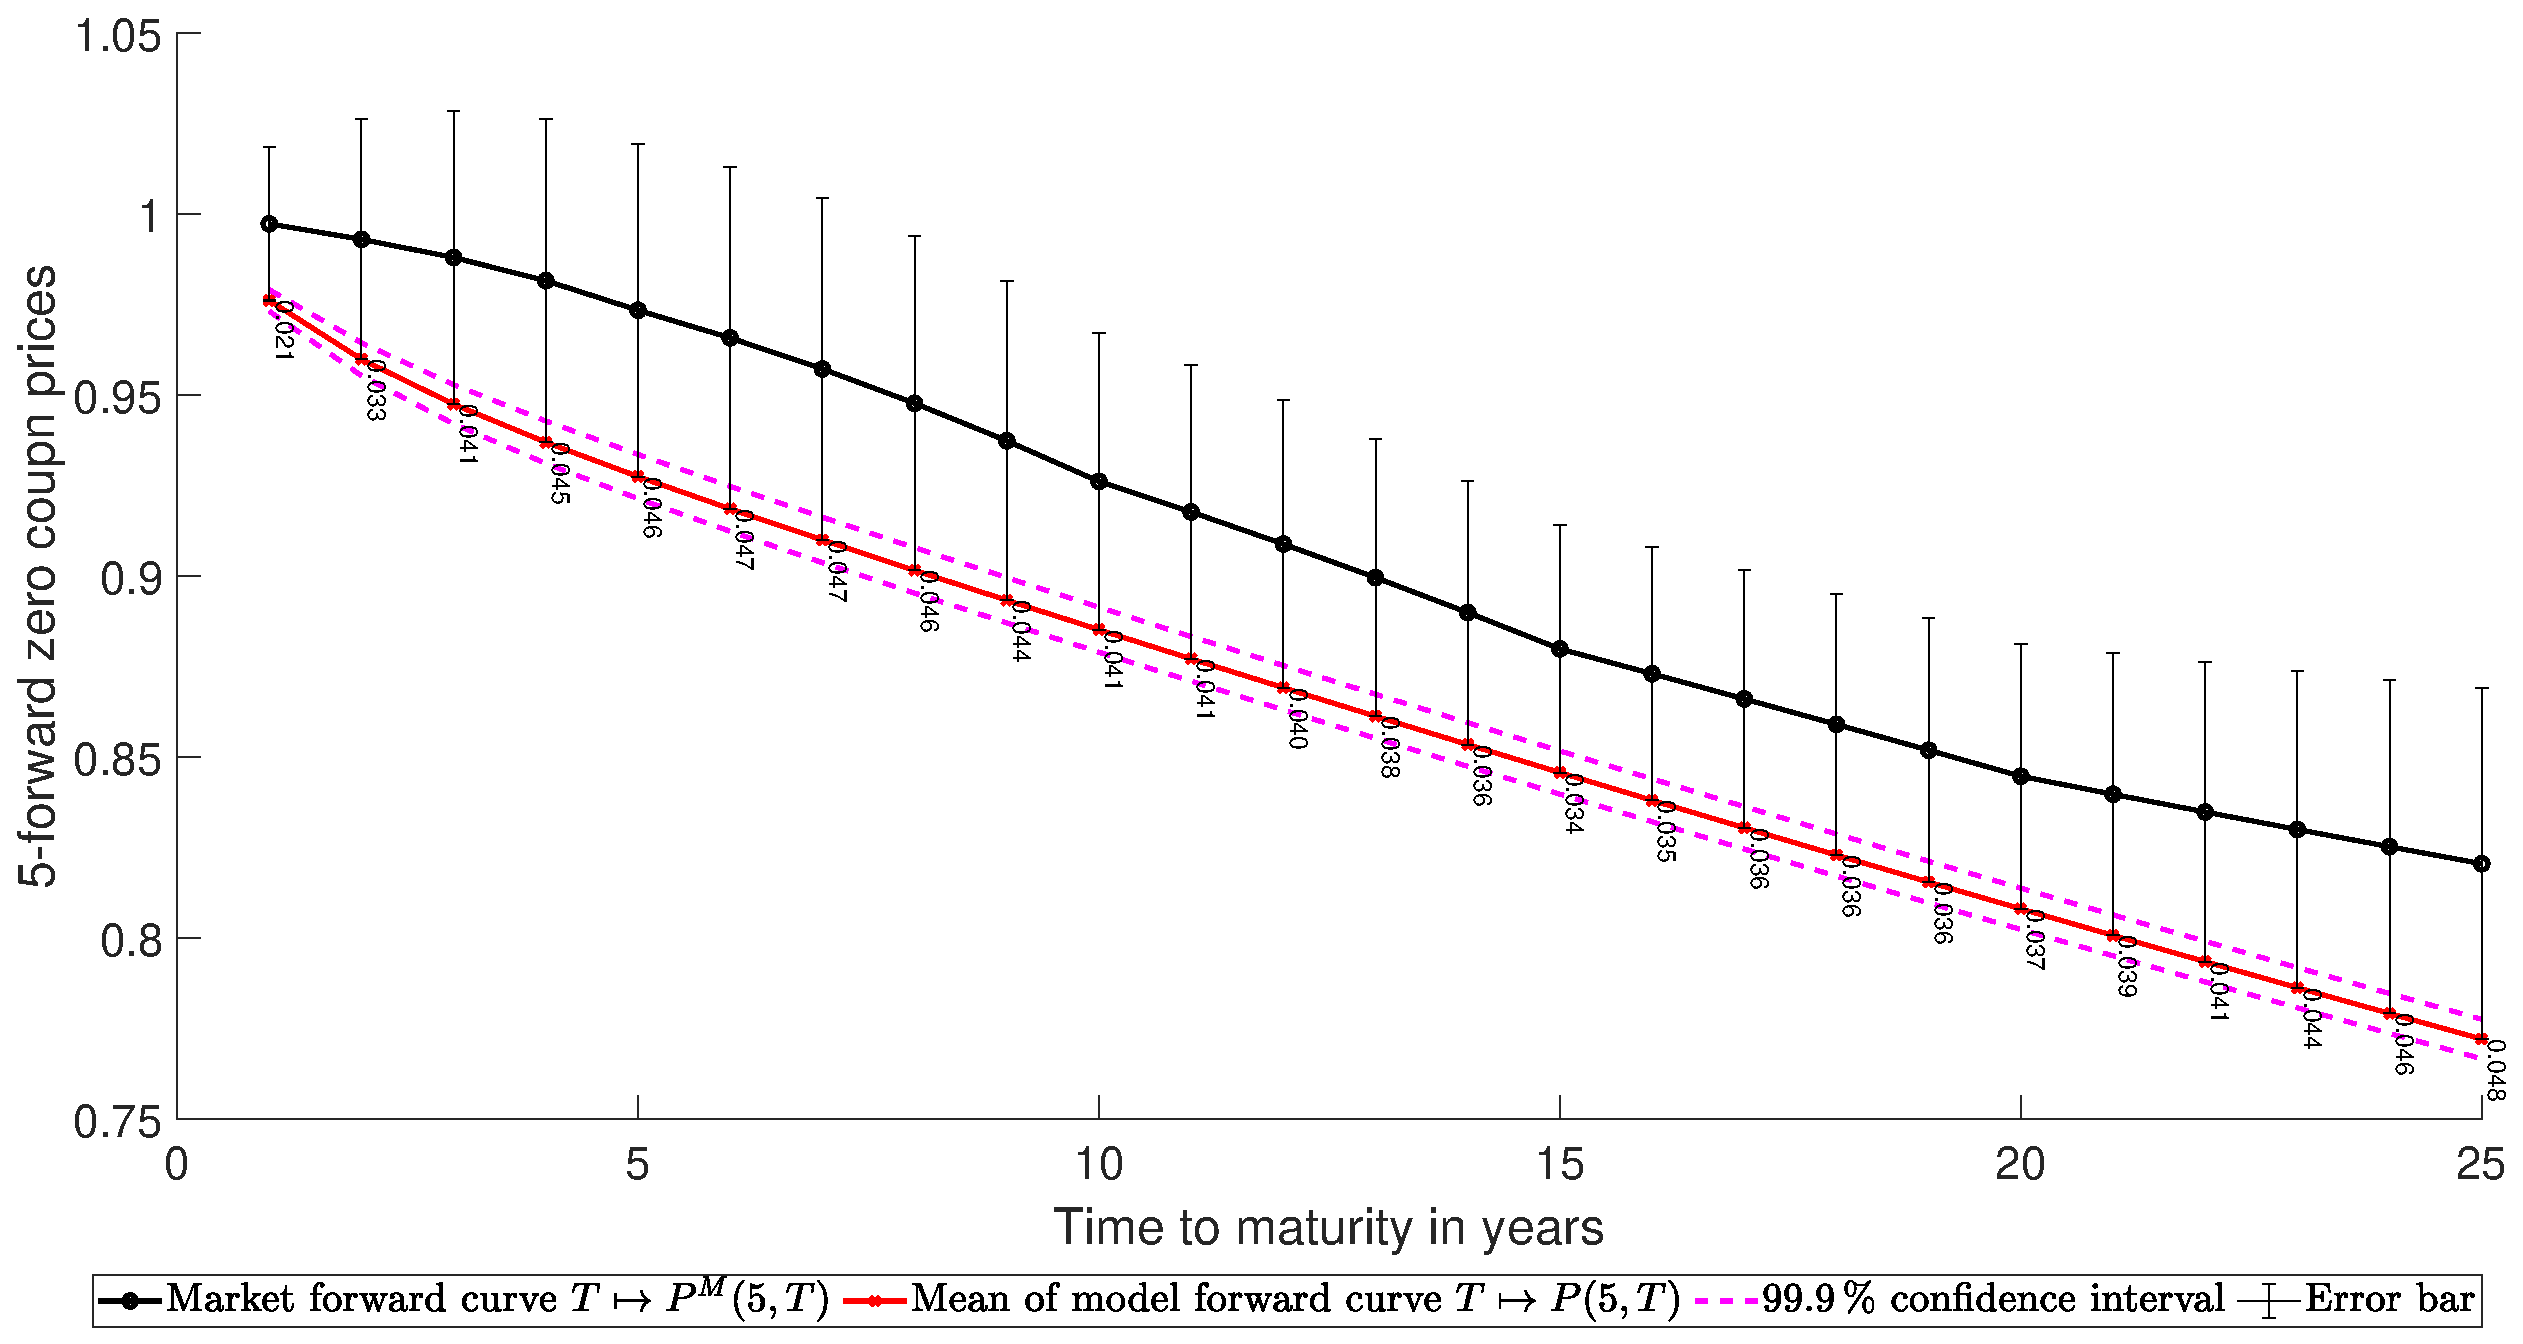
\includegraphics[width=.95\columnwidth]{Forward/F_A_3}
\end{landscape}

\subsection{Plots of Forward Zero-Coupon Prices}
	\begin{landscape}
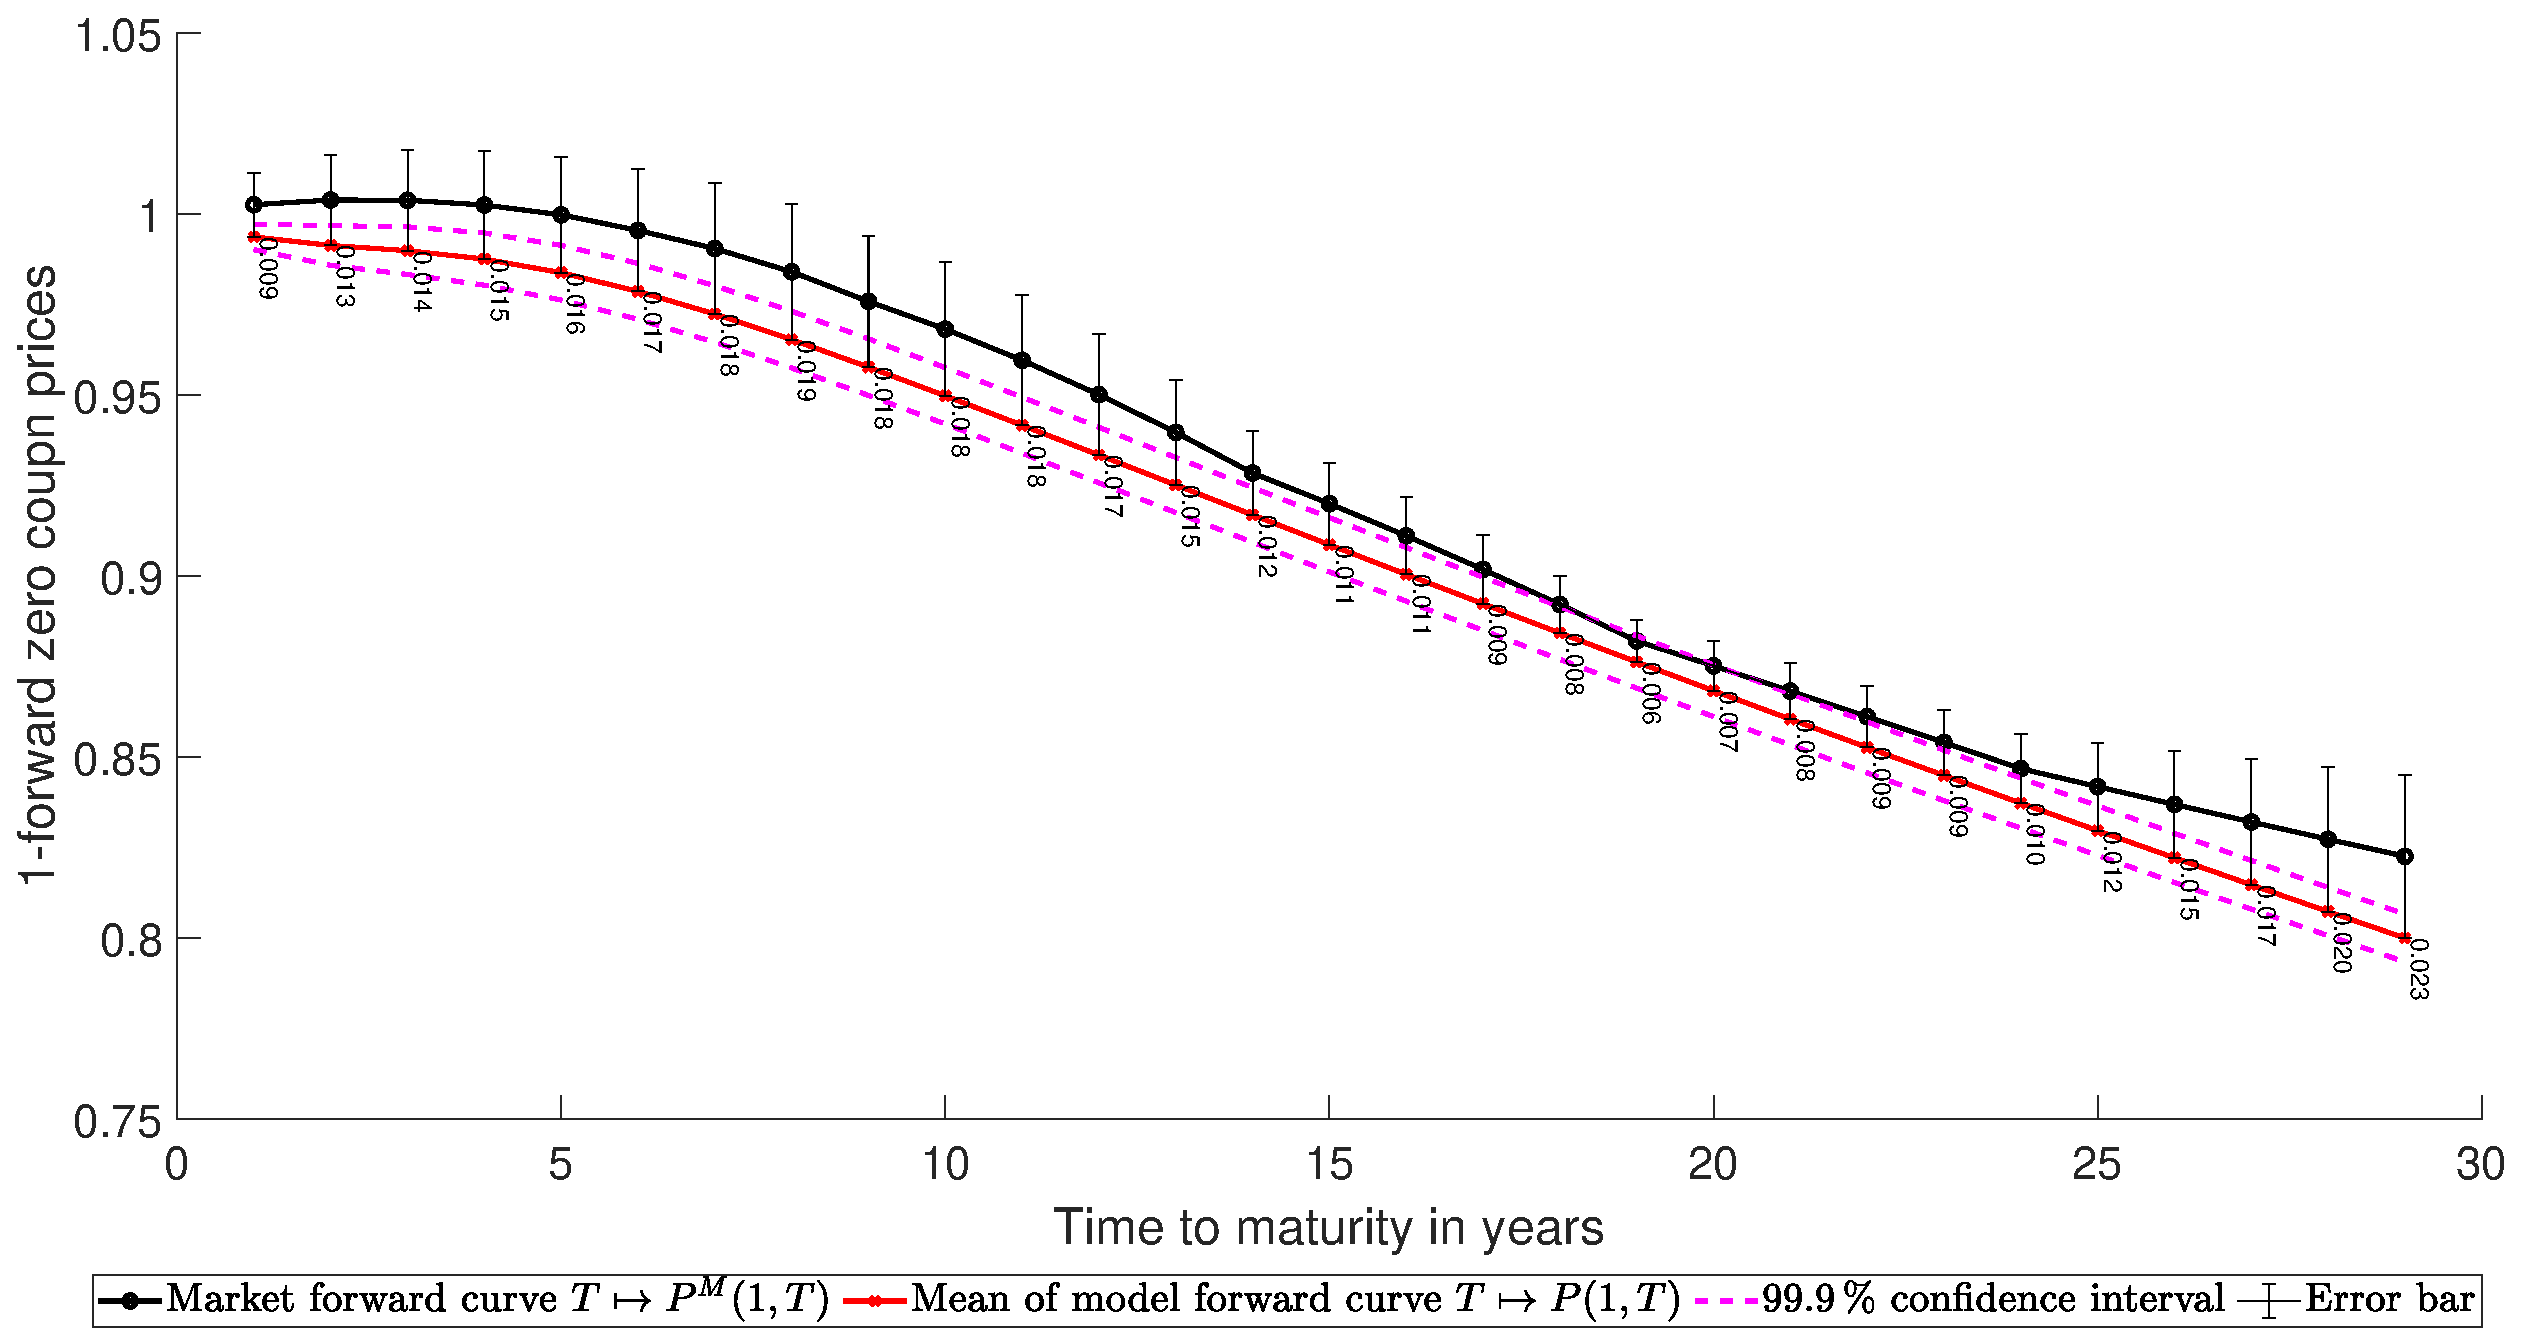
\includegraphics[width=.95\columnwidth]{Forward/F_A_1}
\end{landscape}
\begin{landscape}
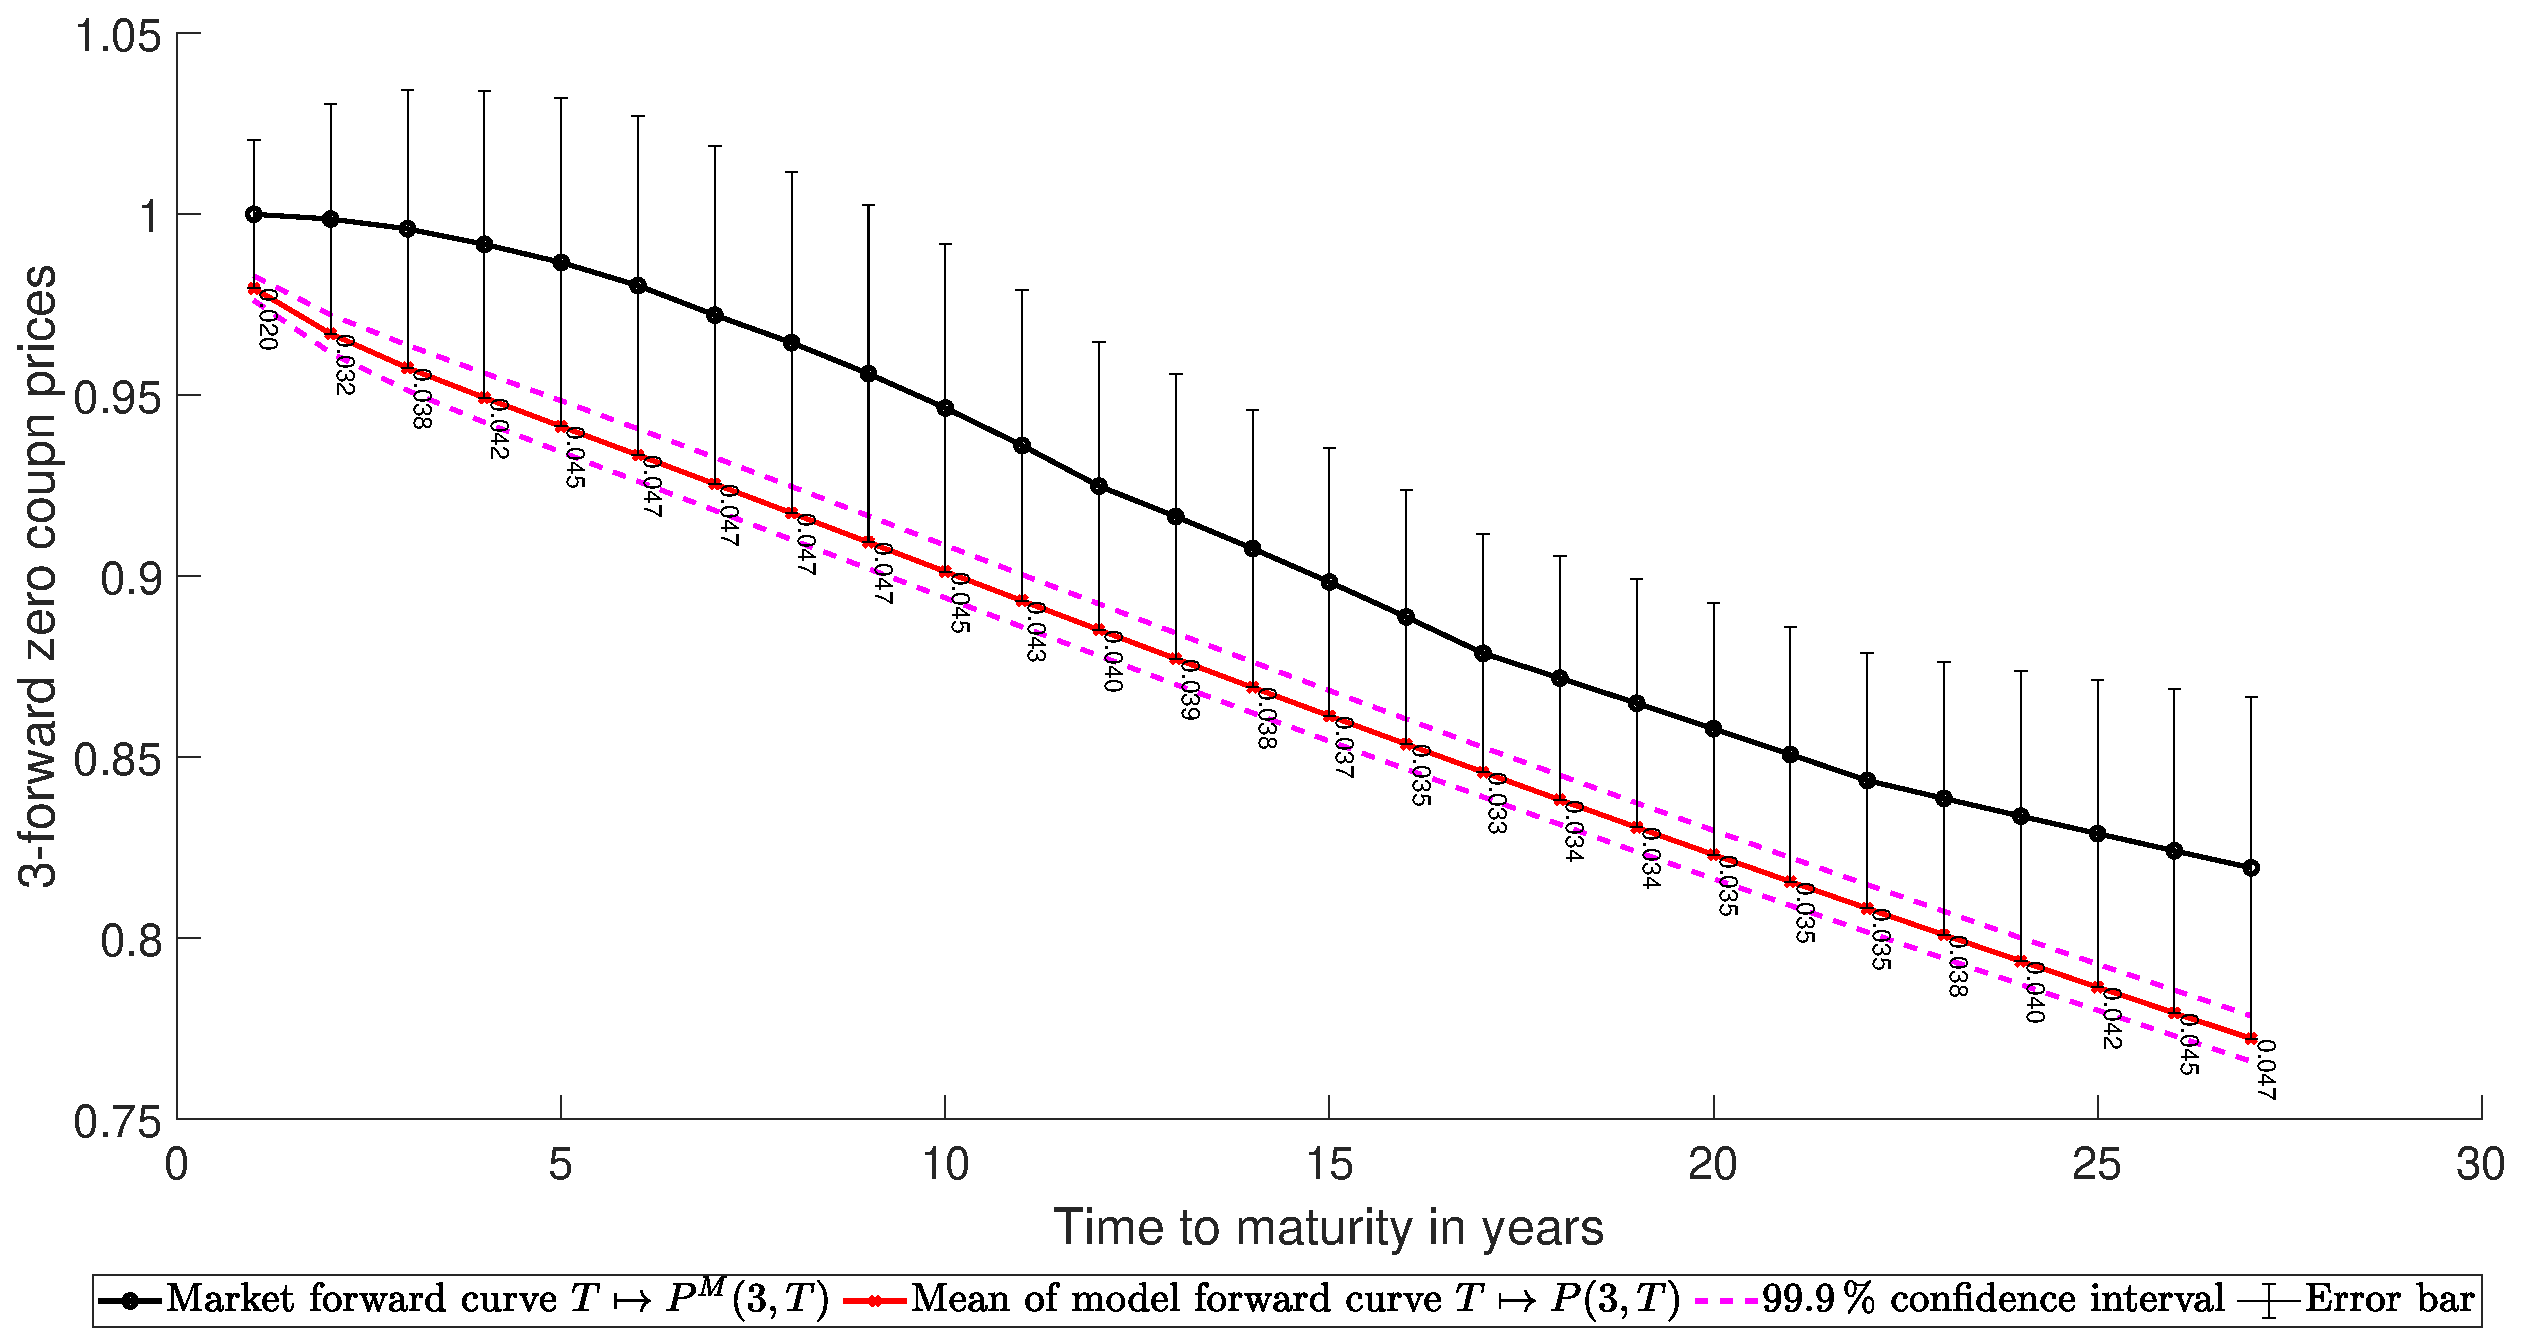
\includegraphics[width=.95\columnwidth]{Forward/F_A_2}
\end{landscape}
\begin{landscape}
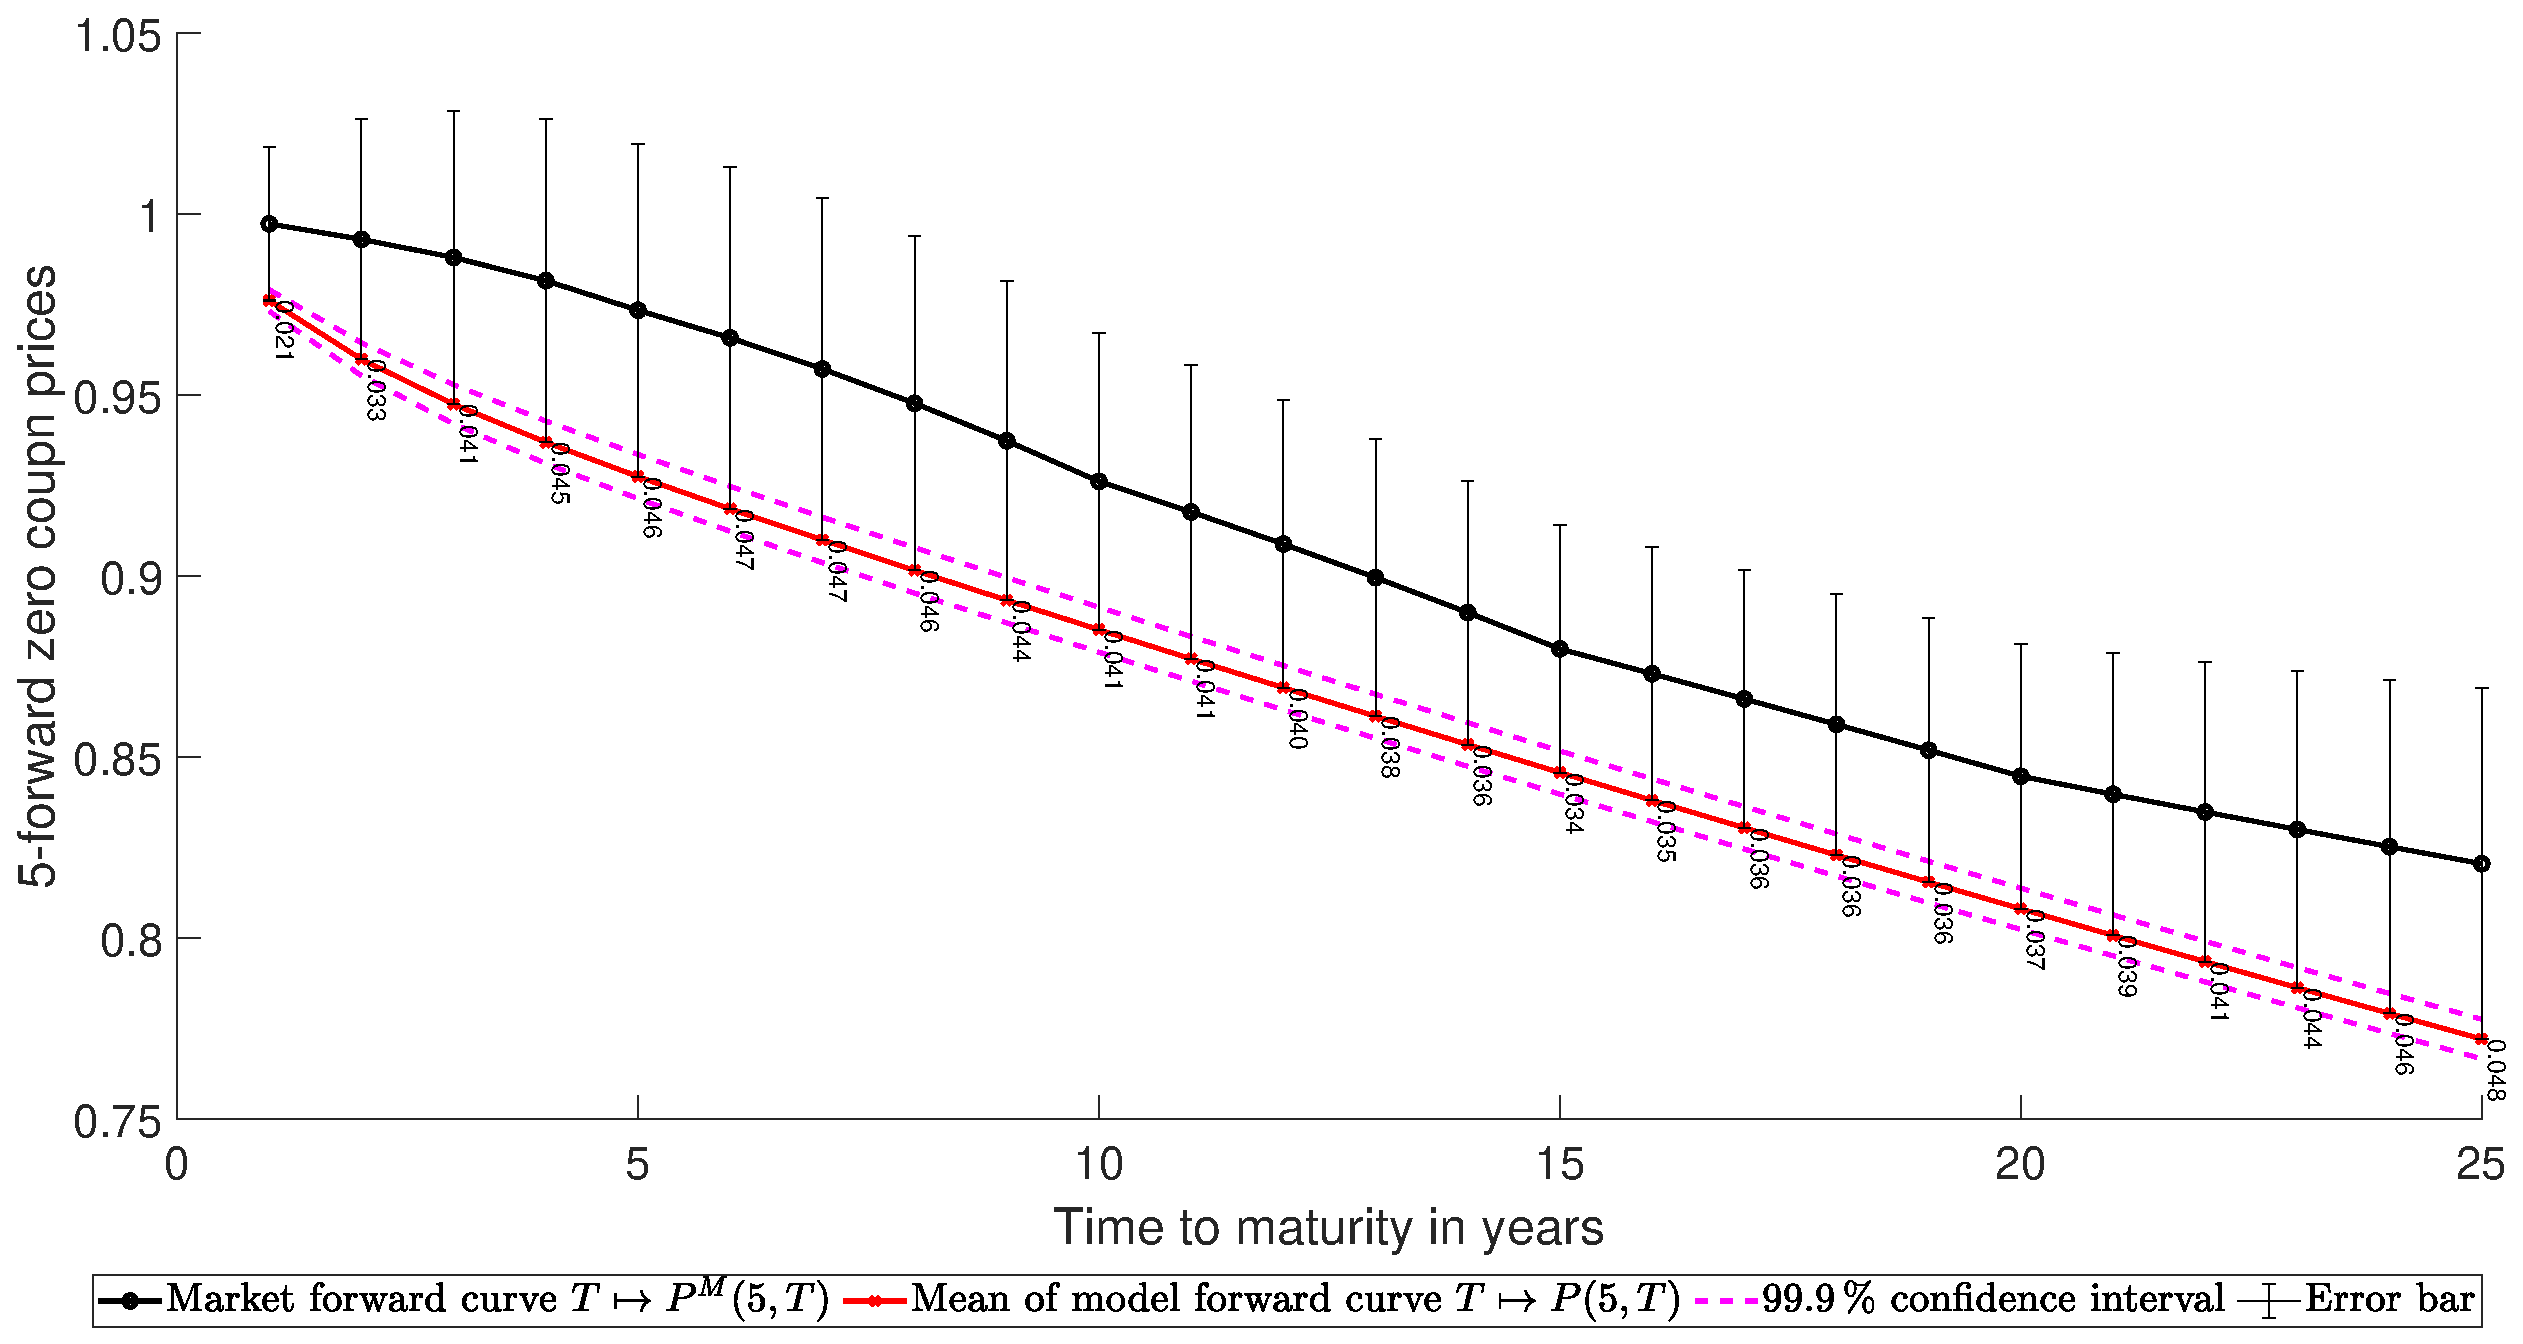
\includegraphics[width=.95\columnwidth]{Forward/F_A_3}
\end{landscape}

\appendix
\section{Market Data}
	\newcommand{\marketDataA}{
\renewcommand{\arraystretch}{1}
\begin{tabular}{|*{3}{c}|}
\hline
Maturity (in years) & Zero rate (in \%) & Zero-coupon price\\
\hline
$0.0833333333333333$ & $-0.469999993219972$ & $  1.0004001991529$ \\
$             0.25$ & $-0.388000020757318$ & $ 1.00096969387991$ \\
$              0.5$ & $-0.324999983422458$ & $ 1.00163343819125$ \\
$             0.75$ & $-0.314333918504417$ & $ 1.00237481461989$ \\
$                1$ & $-0.322000007145107$ & $ 1.00323926670136$ \\
$             1.25$ & $-0.323286440253412$ & $ 1.00405360258242$ \\
$              1.5$ & $-0.316161320131414$ & $ 1.00476558980205$ \\
$             1.75$ & $-0.303842297803669$ & $ 1.00535001652119$ \\
$                2$ & $-0.289547047577798$ & $ 1.00582418019158$ \\
$             2.25$ & $-0.275860329135469$ & $ 1.00623288634409$ \\
$              2.5$ & $-0.262835313503729$ & $   1.006604855007$ \\
$             2.75$ & $-0.249892233800608$ & $ 1.00691299093433$ \\
$                3$ & $-0.236451346427202$ & $ 1.00713375064174$ \\
$             3.25$ & $-0.222084053437044$ & $ 1.00725039326453$ \\
$              3.5$ & $-0.20696636298112$ & $ 1.00728054250496$ \\
$             3.75$ & $-0.191425434683623$ & $ 1.00721781901104$ \\
$                4$ & $-0.175788428168744$ & $ 1.00706740209126$ \\
$             4.25$ & $-0.160311330630236$ & $ 1.00684531811395$ \\
$              4.5$ & $-0.144965462482105$ & $ 1.00655553463348$ \\
$             4.75$ & $-0.129650957156002$ & $ 1.00618948972951$ \\
$                5$ & $-0.114267959725112$ & $ 1.00573933685071$ \\
$             5.25$ & $-0.0987154224631581$ & $ 1.00520062530541$ \\
$              5.5$ & $-0.0828875612342017$ & $ 1.00457454544122$ \\
$             5.75$ & $-0.0666773874613114$ & $ 1.00384671986489$ \\
$                6$ & $-0.0499779242090881$ & $ 1.00300667524933$ \\
$             6.25$ & $-0.0327643402378897$ & $ 1.00205088034181$ \\
$              6.5$ & $-0.0153403983915723$ & $ 1.00099833086134$ \\
$             6.75$ & $0.00190798987986796$ & $0.999871102605028$ \\
$                7$ & $0.0185949131264351$ & $0.998698306220564$ \\
$             7.25$ & $0.0344518735623467$ & $0.997505079039002$ \\
$              7.5$ & $0.0496800311054812$ & $0.996279818846146$ \\
$             7.75$ & $0.0645979575189415$ & $0.995003816465917$ \\
$                8$ & $0.0795242260210216$ & $0.993656440330286$ \\
$             8.25$ & $0.0947347900819295$ & $0.992214008696662$ \\
$              8.5$ & $0.110335148849572$ & $0.990662992494919$ \\
$             8.75$ & $0.126388167535652$ & $0.988997743889118$ \\
$                9$ & $0.142956722993404$ & $0.987213788328959$ \\
$             9.25$ & $0.160050573928316$ & $0.985308478446392$ \\
$              9.5$ & $0.177466994199449$ & $0.983284710270437$ \\
$             9.75$ & $0.194950156980411$ & $0.981173005874126$ \\
$               10$ & $0.212244223803282$ & $0.979004189945635$ \\
$               15$ & $0.473523046821356$ & $0.931543316237289$ \\
$               20$ & $0.611338950693607$ & $0.885166902653398$ \\
$               25$ & $0.652327481657267$ & $0.849865688031976$ \\
$               30$ & $0.640345783904195$ & $0.825611308910539$ \\\hline
\end{tabular}
}

\begin{table}
	\marketDataA
\centering
\caption{Market data containing the zero rate curve and zero coupon curve at 30/12/2019.}
\label{tab:market_dataA}
\end{table}
\section{Market Data}
	\newcommand{\strikeSwaptionA}{
\renewcommand{\arraystretch}{1}
\begin{tabular}{|c|*{5}{c}|}
\hline
\diagbox{Maturity}{Tenor} & 1 & 2 & 5 & 7 & 10 \\
 \hline
$1$ & $-0.260793\,\% $ & $-0.195187\,\% $ & $-0.011405\,\% $ & $0.140129\,\% $ & $0.330514\,\% $ \\
$2$ & $-0.129665\,\% $ & $-0.0782444\,\% $ & $0.139932\,\% $ & $0.273273\,\% $ & $0.449172\,\% $ \\
$5$ & $0.268095\,\% $ & $0.38307\,\% $ & $0.556996\,\% $ & $0.655339\,\% $ & $0.757978\,\% $ \\
$7$ & $0.547079\,\% $ & $0.611571\,\% $ & $0.76683\,\% $ & $0.830788\,\% $ & $0.891069\,\% $ \\
$10$ & $0.880582\,\% $ & $0.907944\,\% $ & $0.967521\,\% $ & $0.988131\,\% $ & $0.992003\,\% $ \\
$15$ & $1.04232\,\% $ & $1.04153\,\% $ & $1.01776\,\% $ & $0.985317\,\% $ & $0.924744\,\% $ \\
$20$ & $0.925377\,\% $ & $0.901441\,\% $ & $0.827386\,\% $ & $0.778437\,\% $ & $0.721445\,\% $ 
\\\hline
\end{tabular}
}

\begin{table}
	\strikeSwaptionA
\centering
\caption{Market data containing the swaption strikes at 30/12/2019.}
\label{tab:strike_swaptionA}
\end{table}
\section{Market Data}
	\newcommand{\marketSwaptionA}{
\renewcommand{\arraystretch}{1}
\begin{tabular}{|c|*{5}{c}|}
\hline
\diagbox{Maturity}{Tenor} & 1 & 2 & 5 & 7 & 10 \\
 \hline
$1$ & $0.000702236$ & $0.00175071$ & $0.00706456$ & $0.0112631$ & $0.0181169$ \\
$2$ & $0.0014433$ & $0.00333027$ & $0.0111956$ & $0.017189$ & $0.0265694$ \\
$5$ & $0.00391314$ & $0.00796766$ & $0.0214221$ & $0.0308074$ & $0.0453508$ \\
$7$ & $0.00521117$ & $0.0104082$ & $0.0268942$ & $0.0380283$ & $0.0548627$ \\
$10$ & $0.00668368$ & $0.0132567$ & $0.0330802$ & $0.045932$ & $0.0651091$ \\
$15$ & $0.00781681$ & $0.0154396$ & $0.0378811$ & $0.0525334$ & $0.0743464$ \\
$20$ & $0.00840243$ & $0.0166069$ & $0.0407885$ & $0.0565876$ & $0.0795953$ 
\\\hline
\end{tabular}
}

\begin{table}
	\marketSwaptionA
\centering
\caption{Market data containing the swaption prices at 30/12/2019.}
\label{tab:market_swaptionA}
\end{table}
